% !TeX spellcheck = en_US


\chapter{Couette流动}
\label{chap:linearized}
\index{linearized Boltzmann equation}

作为最基本的稀薄气体流动之一,对Couette流动的研究有助于我们加深对稀薄气体动力学的了解。在本章中,我们先使用合成迭代加速算法计算全流域的Couette流动,分析速度剖面、切向热流、剪切应力随克努森数的影响。然后着重研究近连续流下的速度滑移边界条件和克努森层形状。


\section{Planar Couette flow}\label{linear_Couette_flow}
\index{Couette flow}
The geometry is the same as that of the Fourier flow, except that the plate at $x_2=-0.5$ moves with a speed $u_{w}$ in the $x_3$ direction, while the  plate at the plate at $x_2=0.5$ moves in the opposite direction with the same speed. When the wall speed is far less than the most probable speed $v_m$, the Boltzmann equation is linearized to Eq.~\eqref{Chapter1_Boltzmann_lin} by choosing $\beta=u_{w}/v_m$. The diffuse BC for the perturbation VDF reflected from the wall is 
\begin{equation}
h(\bm{v},x_2=-0.5)=2v_3f_{eq}, %\quad \text{when} \quad v_2>0, 
\end{equation} while at the channel center $h(v_1,v_2,v_3,x_2=0)=h(v_1,-v_2,-v_3,x_2=0)$. 


Figure~\ref{Fourier_lin} shows the velocity when $\delta_{rp}=0.1$.  The intermolecular potential has a strong influence on the velocity profile, but little influence on the wall shear stress.  

\section{Viscous slip}


%We set the rarefaction parameter to be $\delta_{rp}=100$, so that the  distance between two plates is about 100 times larger than the MFP; thus, the interference between Knudsen layers near each plate is avoided. The molecular velocity $v_2$ is discretized according to Eq.~\eqref{nonuniform_v} with $N_v=128$ and $\imath=5$, while $v_1$ and $v_3$ are discretized by $32\times32$ uniform grids in the range of $[-6,6]$; in the spatial discretization we choose $N_s=500$ in Eq.~\eqref{spatial_d}. In the fast spectral approximation of the linearized Boltzmann collision operator, the integral with respect to the solid angle $\Omega$ is calculated by the Gauss-Legendre quadrature with $M=8$, see Eq.~\eqref{kernel_FSM_modee}. All these measures enable our results holding an accuracy of at least 6 significant digits.

The LBE is solved for the Couette flow between two parallel plates.  When the steady-state solution is obtained, the velocity profile in the bulk region is linearly fitted by $u_{NS}=k_1(x_2-1/2)$ in the dimensionless form, where $k_0$ is the coefficient from the least square fitting. Then the KLF is calculated according to the following equation:
\begin{equation}\label{NS_fit}
u_s\left(\frac{x_2}{\text{Kn}}\right)=\frac{u_{NS}(x_2)-u_1(x_2)}{k_1\text{Kn}},
\end{equation}
and the VSC is calculated as
\begin{equation}\label{slip_coe}
\sigma_P=-\frac{2-k_1}{2\bar{P}},
\end{equation}
where $\bar{P}$ is the wall shear stress. 

%where the Knudsen number is formally defined as $\text{Kn}=\lambda/H=\sqrt{\pi}/2\delta$. 
%Note that the MFP is $\lambda=(\sqrt{\pi}/2)(\mu v_m)/(n_0k_BT_w)$.


%In the numerical simulation, we find that $\delta_{rp}=100$ is accurate enough to recover the KLF and VSC, when compared to the solution of $\delta_{rp}=1000$. However, when $\delta_{rp}=10$, that is, the  distance between two plates is roughly 10 times of the MFP, two Knudsen layers interact with each other, which leads to an inaccurate KLF by using Eq.~\eqref{NS_fit}.




\subsection{Viscous slip coefficient}\label{sec:coe}
\index{viscous slip coefficient}



\begin{table}[t]
	\caption{ The VSC for HS, VHS with $\omega=0.81$, and Maxwell molecules under Cercignani-Lampis BC with different TMAC $\alpha_t$ and EAC $\alpha_n$.}
	\label{table_CL_0}
	\centering
	
	\begin{tabular}{cccccc}
		\hline
		$\alpha_t$	& $\omega$
		&  $\alpha_n=0.25$ & $ 0.5$  &    $0.75$ &    $ 1$\\
		%%	\rowcolor[gray]{.9}
		$0.25$
		& 0.5	& 6.365427  & 6.343336   & 6.324267 &  6.307321  \\
		&0.81	& 6.400178  & 6.372316   & 6.347638 &  6.325202  \\
		&1	    & 6.426786  & 6.394845   & 6.366237 &  6.339971  \\
		%	\rowcolor[gray]{.9}
		$0.5$
		& 0.5	& 2.799516   & 2.785158   & 2.772602 & 2.761338  \\
		&0.81	& 2.829277   & 2.811279   & 2.795092 & 2.780207  \\
		&1		& 2.851688   & 2.831142   & 2.812430 &  2.795028  \\
		
		$0.75$
		& 0.5	& 1.598122   & 1.591127   & 1.584932  & 1.579323 \\
		&0.81	& 1.622629   & 1.613906   & 1.605945  & 1.598540 \\
		&1		& 1.641138   & 1.631215   & 1.622031 &  1.613380  \\
		%	\rowcolor[gray]{.9}
		$1.0$
		& 0.5	& 0.988451   & 0.988451   & 0.988451 & 0.988451 \\
		&0.81	& 1.007717   & 1.007717   & 1.007717 & 1.007717 \\
		&1		& 1.022560   & 1.022560   & 1.022560 &  1.022560  \\
		
		%	\rowcolor[gray]{.9}
		$1.25$
		& 0.5	& 0.615670   & 0.622315   & 0.628343 &  0.633906 \\
		&0.81	& 0.629985   & 0.638188   & 0.645891  & 0.653221 \\
		&1		& 0.641382   & 0.650657   & 0.659514 &  0.668067  \\
		
		%	\rowcolor[gray]{.9}
		$1.5$
		& 0.5	& 0.361248   & 0.374217   & 0.386121 & 0.397213 \\
		&0.81	& 0.371198   & 0.387115   & 0.402275 &0.416866 \\
		&1		& 0.379386   & 0.397328   & 0.414721 & 0.431729  \\
		
		%	\rowcolor[gray]{.9}
		$1.75$
		& 0.5	& 0.174178   & 0.193187   & 0.210840   & 0.227456\\
		&0.81	& 0.180631   & 0.203809   & 0.226193  & 0.247988 \\
		&1.0	& 0.185886   & 0.211919   & 0.237535 &  0.262897  \\
		
		$2$
		& 0.5	& 0.028851   & 0.053665   &0.076984 & 0.099153\\
		&0.81	& 0.032881   & 0.062901   &0.092298  & 0.121255 \\
		&1.0	& 0.035527   & 0.069105   &0.102637 &  0.136246  \\
		\hline
	\end{tabular}\par
	
\end{table}

\index{accommodation coefficient!tangential momentum}
\index{accommodation coefficient!energy}
\index{Boundary condition!Cercignani-Lampis}
\index{Boundary condition!Maxwell}
The LBE is solved with the Cercignani-Lampis BC for HS, VHS with $\omega=0.81$, and Maxwell molecules; results are summarized in Table~\ref{table_CL_0}. When the EAC $\alpha_n$ and the intermolecular potential ($\omega$) are fixed, VSC increases rapidly when  the TMAC $\alpha_t$ decreases. The additional free parameter $\alpha_n$ in the Cercignani-Lampis BC introduces new interesting results. When $\alpha_t<1$, for a fixed $\alpha_t$ and intermolecular potential, the VSC decreases slightly as $\alpha_n$ increases, where the maximum drop in the VSC is less than $2\%$. When $\alpha_t=1$, the Cercignani-Lampis BC is reduced to the fully diffuse one in this problem, and the VSC does not vary with $\alpha_n$. When $\alpha_t>1$, the variation of VSC on $\alpha_n$ reverses when compared to that of $\alpha_t<1$; and it is strongly influenced by $\alpha_n$, especially when $\alpha_t$ is large. For instance, for HS molecules at $\alpha_t=2$, the VSC is increased by more than three times when $\alpha_n$ changes from $0.25$ to $1$. 

For fixed $\alpha_n$ and $\alpha_t$, VSC is insensitive to the intermolecular potentials when $\alpha_t\lesssim1.75$. However, when $\alpha_t$ is close to two (the ``backward'' scattering), the influence of intermolecular potential becomes considerable. For example, when $\alpha_t=2$ and $\alpha_n=1$, Maxwell molecules have a VSC that is about 37\% higher than that for HS molecules.




The VSC can be fitted by a general function as the one used by Lilley \& Sader~\cite{lilley2008velocity} for both diffuse-specular and Cercignani-Lampis BCs:
\begin{equation}\label{CL_fit}
\sigma_P(\alpha)=\frac{a}{\alpha}-b\alpha-c,
\end{equation}
where the fitting coefficients $a,~b$, and $c$ are shown in
Table~\ref{table:slipcoe_fit} for typical inverse power-law intermolecular potentials.

% Figure~\ref{fig:slipCoe_fit} shows that the fitted curve (constructed from the data when $\alpha\geq0.2$) can accurately predict the VSC even in the limit $\alpha\rightarrow 0$. For instance,  when the TMAC is 0.05, relative differences between the fitted VSC and the LBE solutions are less than $0.1\%$ for both diffuse-specular and Cercignani-Lampis BCs.


\begin{table}[t]
	\caption{Fitting coefficients in Eq.~\eqref{CL_fit} for HS, VHS with $\omega=0.81$, and Maxwell molecules under the diffuse-specular and Cercignani-Lampis BCs. }
	\label{table:slipcoe_fit}
	\centering
	
	\begin{tabular}{ccccccc}
		\hline
		BC &		$\alpha_n$ & $\omega$
		&  $a$ & $b\cdot 10$  &   $c$   \\
		\hline
		
		Diffuse-specular &	 n/a	& 0.5
		& 1.773  & 1.1660  &  0.6687   \\
		& n/a	& 0.81
		& 1.773  & 1.4270  &  0.6238   \\
		& n/a	& 1
		& 1.773  & 1.6370  &  0.5885   \\
		Cercignani-Lampis &		$0.25$ & 0.5
		& 1.774  & 0.7266  &  0.7127   \\
		&	& 0.81
		& 1.775  & 0.8889  &  0.6781   \\
		&	& 1
		& 1.776  & 1.0130  &  0.6516   \\
		
		Cercignani-Lampis &		$0.5$ & 0.5
		& 1.773  & 0.4772 &  0.7367 \\
		&	& 0.81
		& 1.774  & 0.5867  &  0.7069   \\
		&	& 1
		& 1.774  & 0.5742  &  0.6837  \\
		
		Cercignani-Lampis &		$0.75$ & 0.5
		& 1.772   & 0.2434  &  0.7597   \\
		&	& 0.81
		& 1.773  & 0.2915  &  0.7358  \\
		&	& 1
		& 1.773  & 0.3373  &  0.7164  \\
		%	\rowcolor[gray]{.9}
		Cercignani-Lampis &		$1.0$ &0.5
		& 1.772   &0.0218    & 0.7818 \\
		&	& 0.81
		& 1.766  & 0.0543  &  0.7370   \\
		&	& 1
		& 1.772  & 0.0000  &  0.7499  \\
		\hline
	\end{tabular}\par
	
\end{table}


%\begin{figure}[t]
%	\begin{centering}
%		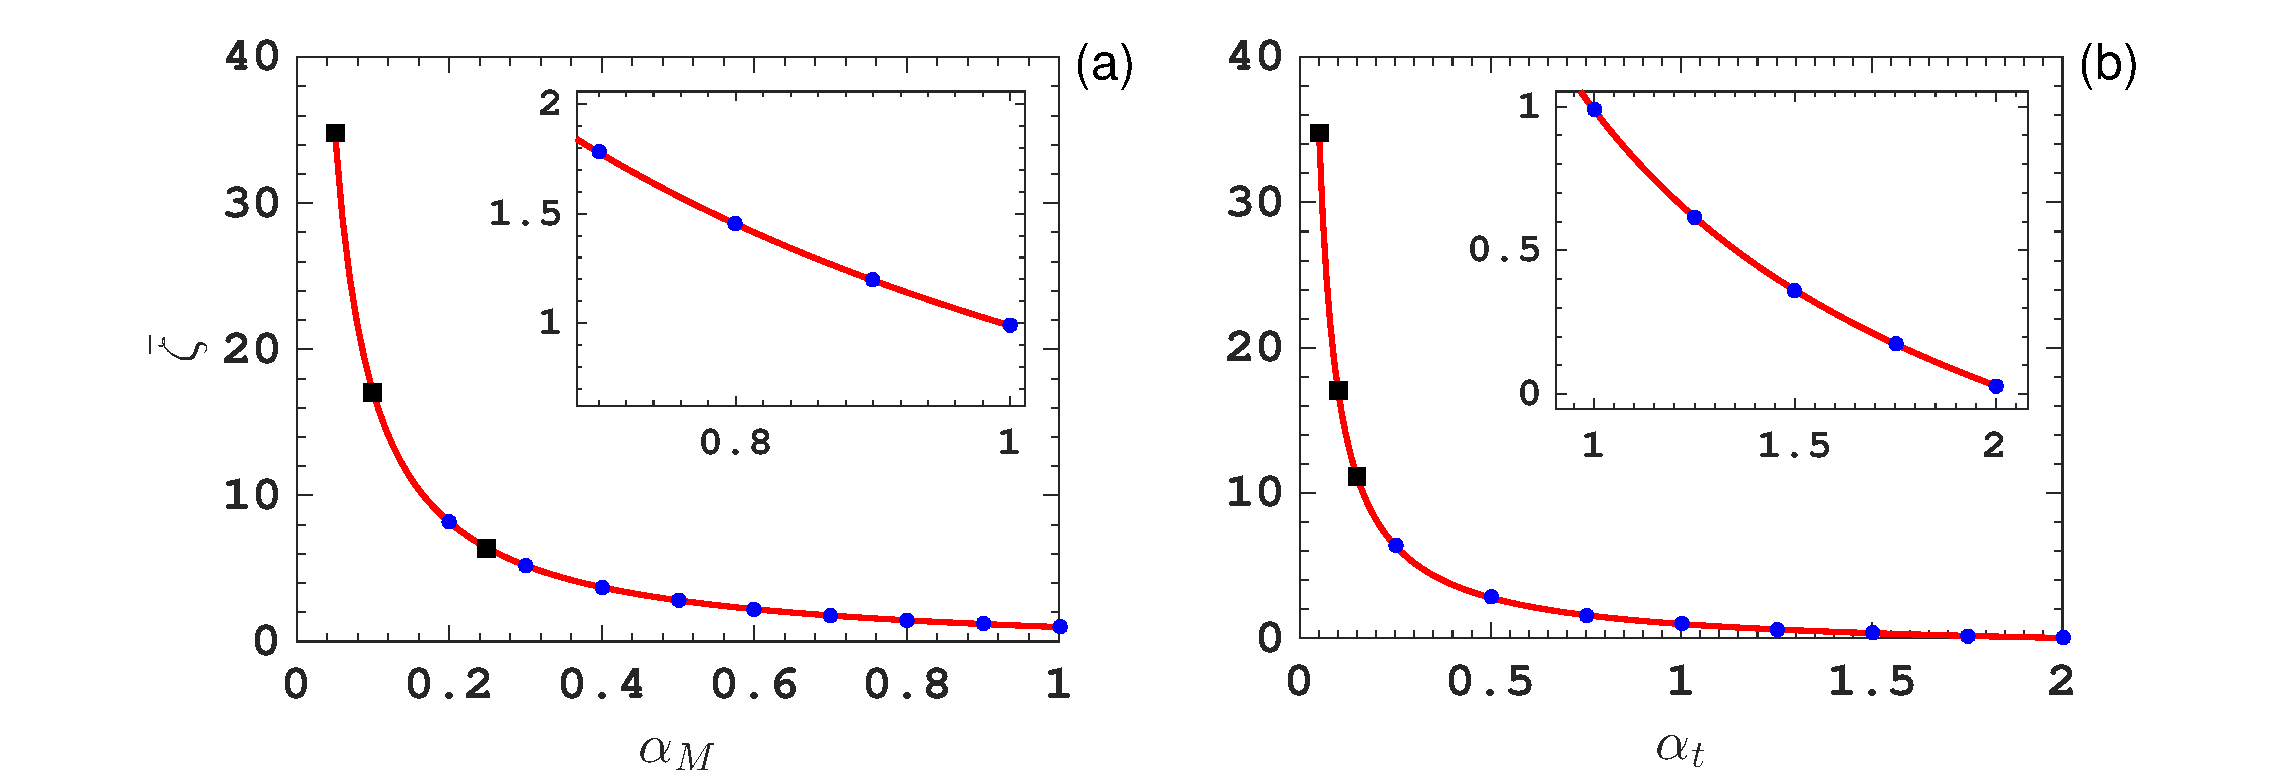
\includegraphics[width=1\textwidth]{SlipJump/IMG/slip_coe_fit}
%		\par\end{centering}
%	\caption{ The VSC as a function of the effective TMAC $\alpha$ for HS molecules, when the (a) diffuse-specular BC and (b) Cercignani-Lampis BC with $\alpha_n=0.25$  are used. Solid lines: the numerical fitting of Eq.~\eqref{CL_fit} using the data from the LBE solutions (circles). Squares: the data from the LBE but no used for fitting. Note that other values of $\alpha_n$ and other types of intermolecular potentials show a similar behavior.
%	}
%	\label{fig:slipCoe_fit}
%\end{figure}




\subsection{Knudsen layer function }\label{sec:knudsenlayer}
\index{Knudsen layer function!Couette}
%
%The KLF is investigated to assess the influence of intermolecular potentials and gas-kinetic BC on the structure of the Knudsen layer. In particular, the KLF from the constant shear profile (Fig.~\ref{fig:kramers_dia}) in the Knudsen layer is studied.




The structure of the Knudsen layer provides a critical information to formulate the effective viscosity. Lockerby \textit{et al.} first proposed a curve-fitted approximation to the Knudsen layer function (KLF) as~\cite{lockerby2005capturing}
\begin{equation}\label{eq:loc_vis}
u_s\left(x\right)\approx\frac{7}{20(1+x)^2},
\end{equation}
where $x$ is the distance to the solid surface normalized by the MFP $\lambda$. It is found that the Navier-Stokes equations with the effective viscosity can predict the velocity profiles in Poiseuille and Couette flows, up to $\text{Kn}=0.4$. Later, by fitting the data from LBE solution of HS gas and the DSMC for Couette flow~\cite{ohwada1989numerical}, Lilley~$\&$~Sader obtained a power-law KLF~\cite{lilley2007velocity,lilley2008velocity}:
\begin{equation}
u_s\left(x\right)=u_s(0)-Cx^n,
\end{equation}
where $C$ is a constant and the exponent $n\approx0.82$. Despite the fact that the fitting is carried out in the region $0.1{\lesssim}x\lesssim1$, they predicted the power-law divergence of the velocity gradient in the vicinity of solid surface, that is, $du_s/dx\rightarrow\infty$ as $x\rightarrow0$.


%\cite{lockerby2005usefulness} also proposed an exponential type of KLF by solving {\color{red}the} high-order hydrodynamic equations.

The singular behavior of velocity gradient at the planar surface is rigorously proved by Takata \& Funagane, when analyzing the thermal transpiration based on the LBE of HS molecules~\cite{takata2013singular}. Instead of the power-law divergence, they found logarithmic divergence of velocity gradient; that is, the spatial singularity is not stronger than $\ln{}x$ in the vicinity of solid surface. This conclusion is confirmed by Jiang \& Luo who, through the asymptotic analysis of BGK  model~\cite{bhatnagar1954model}, found that the velocity profile of Couette flow near the solid surface can be described by the following power series~\cite{lilley2007velocity,lilley2008velocity}:
\begin{equation}\label{eq:vel_fit}
u_s(x)=\sum_{n=0}^{N}\sum_{m=0}^{M}c_{n,m}x^n(x\ln{x})^m, \quad{} x\rightarrow0. %N,M \in \mathbb{Z}^+_0.
\end{equation}
%where four fitting coefficients $c_{n,m}$ are given on the basis of the BGK model, when $x<1.5\times10^{-7}$.

\begin{figure}[t]
	\centering
	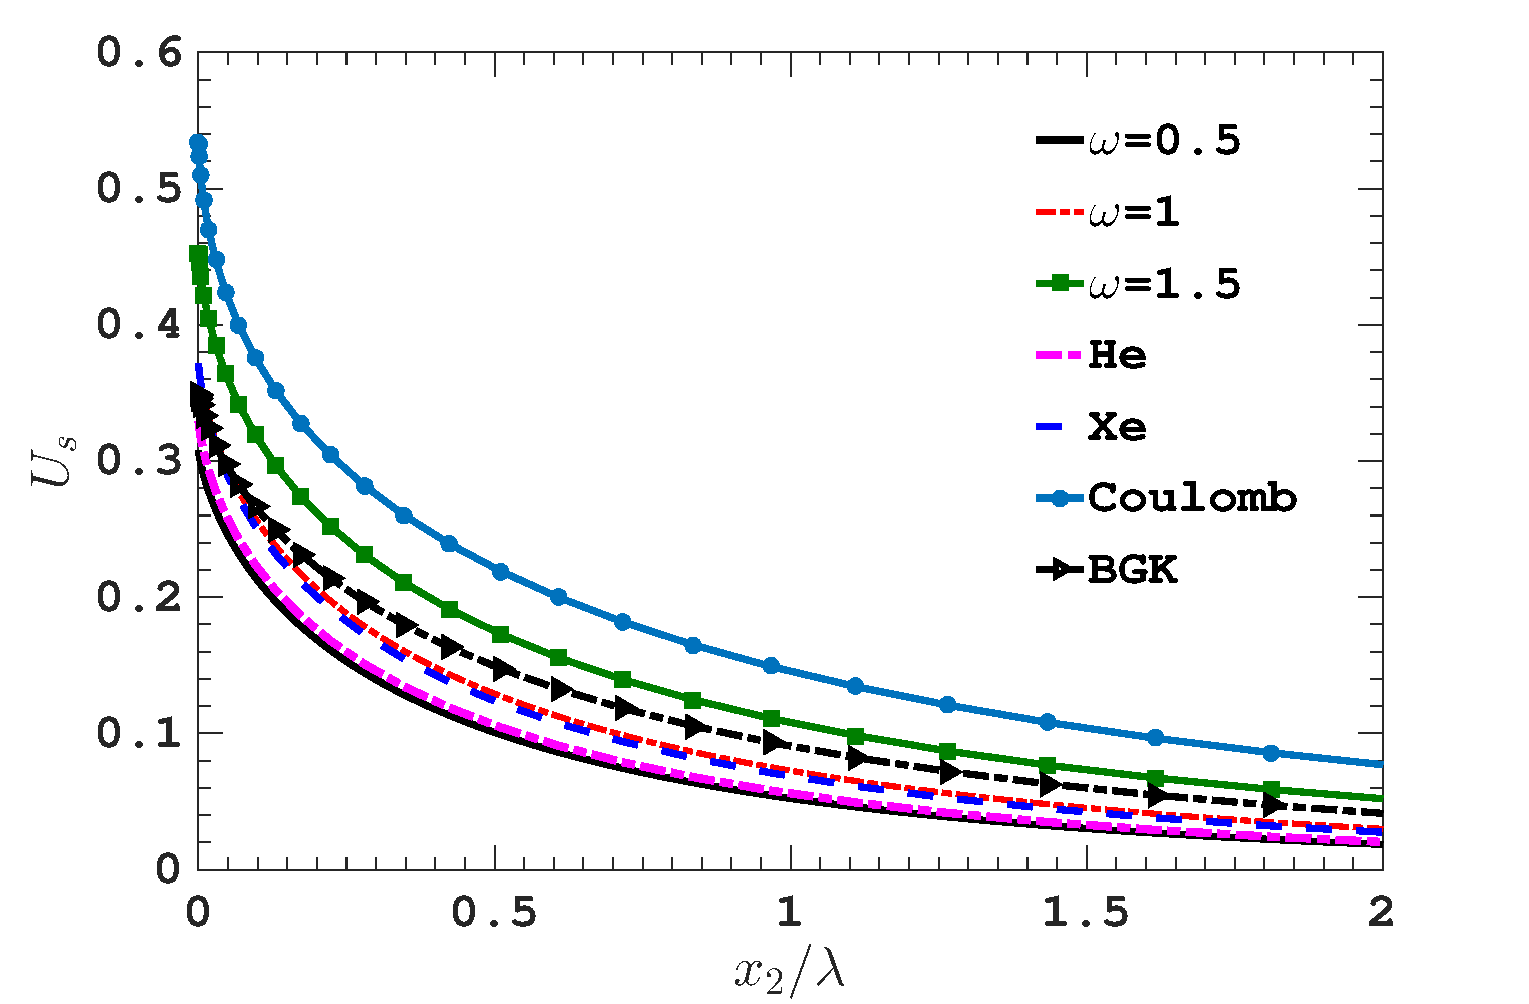
\includegraphics[width=0.7\textwidth]{SlipJump/IMG/vel_def_omega}
	\caption{ KLFs from the LBE solutions for the inverse power-law potentials, the Lennard-Jones potentials of Helium and Xenon when the gas temperature is $300$K, and the shielded Coulomb potential of charged molecules when $\epsilon=k_BT_w$. The result from BGK equation is also included for comparison. The diffuse BC is used.  }
	\label{fig:vel_def_omega}
\end{figure}





\subsubsection{Influence of intermolecular potential}


Figure~\ref{fig:vel_def_omega} illustrates the KLFs obtained from the LBE with the  diffuse BC, for the inverse power-law potential, the Lennard-Jones potential~\eqref{Lennard_Jones_chapter} of helium and xenon, and the shielded Coulomb potential~\eqref{Coulomb_sheiled}. For the inverse power-law potential, the KLF increases with the viscosity index in the whole Knudsen layer. For the Lennard-Jones potential, the KLF of xenon molecules is larger than that of helium, but the results of both helium and xenon lie between those of HS and Maxwell molecules. This is comprehensible because the effective viscosity indexes of helium and xenon at a temperature of $300$K are 0.66 and 0.85~\cite{Bird1994}, respectively. The KLF predicted by the BGK is even larger than that from the Maxwell molecules, but is smaller than that of $\omega=1.5$ where the gas molecules interact with soft potentials. The shielded Coulomb potential has the largest KLF, since its effective viscosity is close to 2.5~\cite{CE}.

\index{power-law potential}
\index{Lennard-Jones potential}

Thus, contrary to the VSC whose value is insensitive to the intermolecular potential, the KLF is strongly affected by the intermolecular potential. That is, when the effective viscosity index increases, (i) the value of the KLF increases, and (ii) the KLF decays more slowly, or equivalently, the Knudsen layer becomes wider. For example, at the solid surface, the relative difference between KLFs of Maxwell and HS molecules is approximate $20\%$, and that between the shielded Coulomb and HS potentials \index{shielded Coulomb potential} reaches 60\%. Relative differences at distances one to two MFP away from the solid surface are even larger, say, when $x_2/\lambda=2$ the value of the KLF of the shielded Coulomb potential is about 4 times of that of HS potential. On the other hand, when $u_s$ is decreased to 0.01 of its value at the solid surface, the corresponding distances to the solid surface for the HS and Maxwell molecules are about $2.7\lambda$ and $3.5\lambda$, respectively.  



\subsubsection{Influence of boundary condition}


\begin{figure}[t]
	\centering
	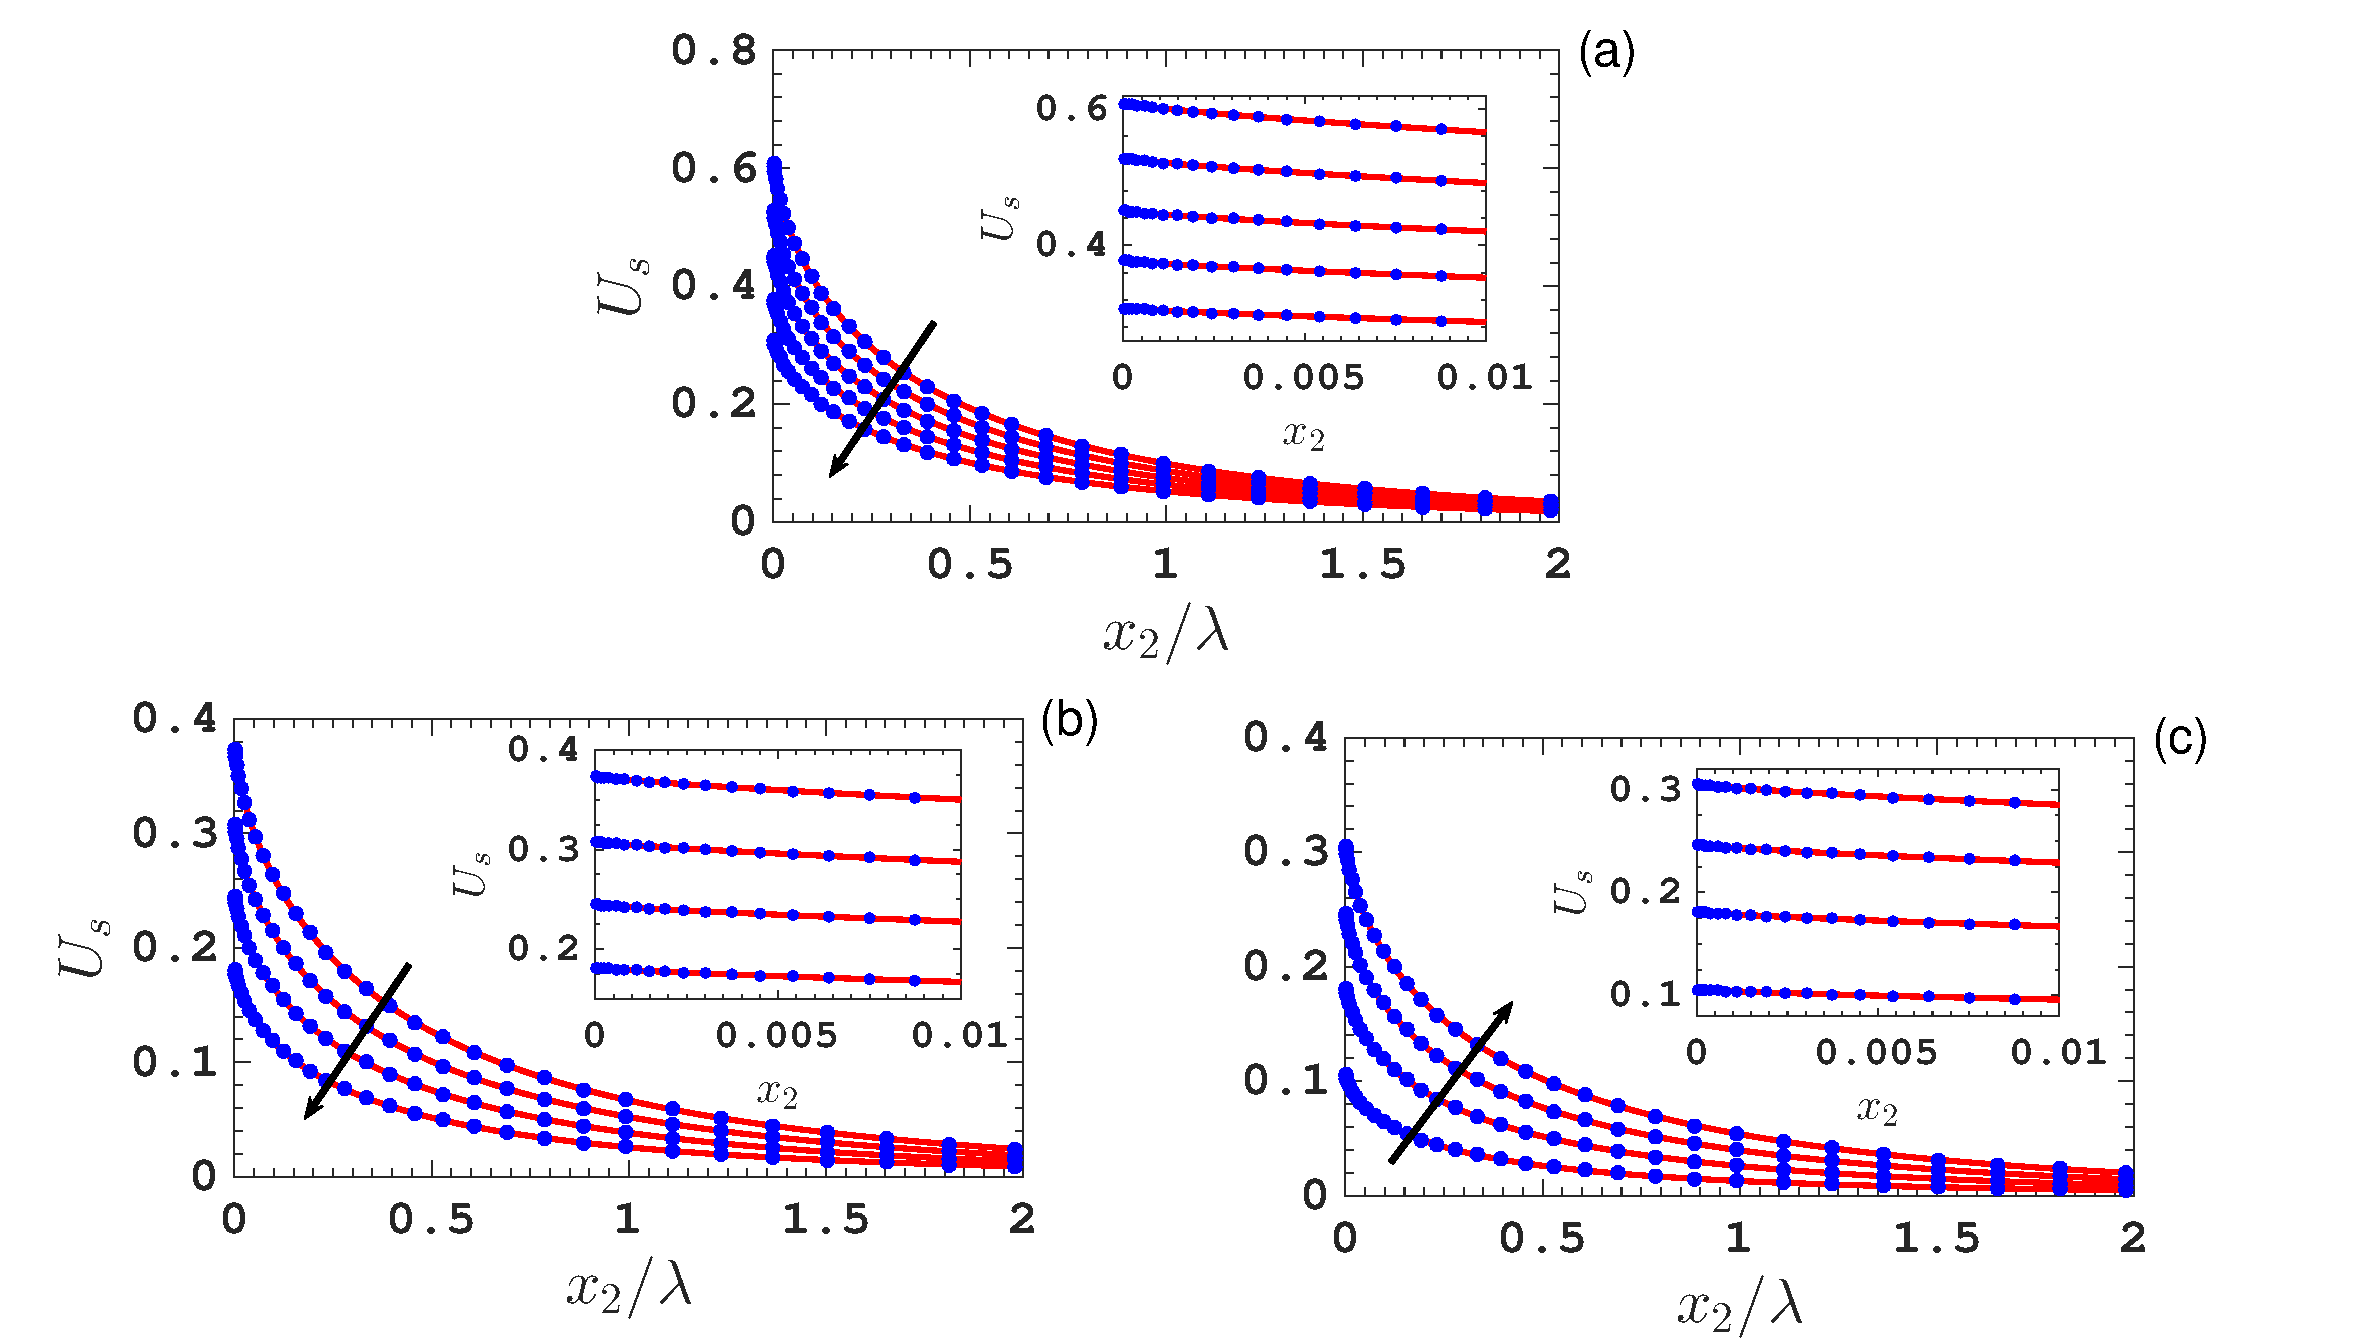
\includegraphics[width=1\textwidth]{SlipJump/IMG/vel_def_CL_Max}
	%\\
	%	\includegraphics[width=0.5\textwidth]{max_hs_rescale_vel_def.eps}
	\caption{The KLF for HS molecules. (a) The diffuse-specular BC. Along the arrow,   $\alpha_M=0.2,0.4,0.6,0.8,1$. (b) The Cercignani-Lampis BC with $\alpha_n=0.25$. Along the arrow, $\alpha_t=0.5,~1,~1.5$ and 2. (c) The Cercignani-Lampis BC with $\alpha_t=2$. Along the arrow, $\alpha_n=0.25,~0.5,~0.75$ and 1. Dots: LBE solutions. Solid lines: fitted curves using Eq.~\eqref{eq:vel_fit} with $M,N=2$. Insets: zoomed regions in the vicinity of the solid surface. %(Last row) The rescaled KLF $u_s/u_s(x_2=0)$ for $\alpha_M=0.2$ and 1, when the diffuse-specular BC are used. For clarity, results at other values of $\alpha_M$ are not shown. Inset: the relative difference ($R\%$) of $u_s/u_s(x_2=0)$ for various $\alpha_M$ compared to that of $\alpha_M=0.2$. 
	}
	\label{fig:vel_def_cl_max}
\end{figure}

For the sake of clarity, we only focus on  HS molecules. The diffuse-specular BC is shown in Fig.~\ref{fig:vel_def_cl_max}(a), where the KLF increases as $\alpha_M$ decreases. Typical KLFs under Cercignani-Lampis BC are plotted in Figs.~\ref{fig:vel_def_cl_max}(b) and~(c). When $\alpha_n$ is fixed, for example, for $\alpha_n=0.25$, the KLF decreases as $\alpha_t$ increases. The relative reduction in $u_s(x_2=0)$ is about $40\%$ when $\alpha_t$ rises from 0.25 to 1. However, the variation of the KLF with respect to $\alpha_t$ becomes weaken as $\alpha_n$ increases, such that at $\alpha_n=1$ the reduction in $u_s(x_2=0)$ with $\alpha_t$ falls below $3\%$. When $\alpha_t$ ($\neq1$) is fixed, the influence of $\alpha_n$ on the KLF becomes larger when $\alpha_n$ increases. And the greater the TMAC $\alpha_t$ exceeds 1, the more pronounced the change in the KLF with $\alpha_n$. As an example, when $\alpha_t=2$, the KLF is increased by three times, as the $\alpha_n$ varies from 0.25 to 1, see Fig.~\ref{fig:vel_def_cl_max}(c).  


%In other words, the Cercignani-Lampis BC with one more accommodation coefficient can present more realistic physical phenomena than the diffuse-specular BC.
%
%\begin{table}[pt]
%	\caption{ Fitted coefficients  corresponding to Eq.~\eqref{eq:vel_fit} with $M,N=2$ for the KLF obtained from the LBE with HS, VHS with $\omega=0.81$, and Maxwell molecules, when the diffuse-specular BC is used.}
%	\label{table_df_coe}
%	\centering
%	
%	\begin{tabular}{ccccccccccl}
%		\hline
%		$\omega$	& $\alpha_M$
%		&  $c_{0,0}$ & $c_{0,1}$  &   $c_{0,2}$ &   $c_{1,0}$ &   $c_{1,1}$ &   $c_{1,2}\cdot10$ &   $c_{2,0}$ &   $c_{2,1}$ &   $c_{2,2}\cdot 10^{2}$   \\
%		\hline
%		%%	\rowcolor[gray]{.9}
%		$0.5$
%		& 0.1 & 0.6502  & 1.2720  & -0.3624& 1.4640  & 0.9950  & -0.6074  & -2.0090  &  0.1593 &0.2246   \\
%		& 0.2 & 0.6084  & 1.1760  & -0.3257& 1.3260  & 0.9093  & -0.5358  & -1.8360  & 0.1410 &0.1967   \\
%		& 0.3 & 0.5675  &1.0830   & -0.2915& 1.1970  & 0.8283  & -0.4699  & -1.6720  & 0.1241 &0.1712   \\
%		& 0.4 & 0.5277  &0.9941   & -0.2598& 1.0760  & 0.7517  & -0.4095  &-1.5170   & 0.1085 & 0.1479  \\
%		& 0.5  & 0.4889 &0.9091   &-0.2302 & 0.9630  & 0.6792  &  -0.3543 & -1.3710 & 0.0943 &0.1267  \\
%		& 0.6  & 0.4509 &0.8277   &-0.2029 & 0.8570  & 0.6108  &  -0.3040 & -1.2330  & 0.0813 &0.1075  \\
%		& 0.7  & 0.4139 & 0.7498  &-0.1776 & 0.7582  &0.5463   &  -0.2585 & -1.1030  & 0.0695 &0.0902  \\
%		& 0.8  & 0.3778 & 0.6752  &-0.1543 & 0.6661  &0.4856   &  -0.2173 & -0.9805 & 0.0588 &0.0748  \\
%		& 0.9  & 0.3424 & 0.6038  &-0.1328 & 0.5805  &0.4284   &  -0.1805 & -0.8652 & 0.0492 &0.0610 \\
%		& 1.0  & 0.3079 & 0.5356  &-0.1132 & 0.5012  & 0.3746 & -0.1480   & -0.7568 &0.0406 &0.0489  \\
%		$0.81$
%		& 0.1 & 0.7436 & 1.6500   & -0.6657& 2.3940  &  1.4840 & -1.3430 &-3.0070 & 0.3430 &0.5216 \\
%		& 0.2 & 0.6935 & 1.5130   & -0.5949& 2.1550  &  1.3470 & -1.1840 &-2.7270 & 0.3030 &0.4571 \\
%		& 0.3 & 0.6450  & 1.3840   & -0.5294& 1.9330  &  1.2180 & -1.0380 &-2.4640& 0.2664 & 0.3983 \\
%		& 0.4 & 0.5980  & 1.2610   & -0.4691& 1.7270  &  1.0980 & -0.9046 &-2.2190& 0.2329 & 0.3449 \\
%		& 0.5 & 0.5523 & 1.1450   & -0.4135& 1.5360  & 0.9858 &-0.7836  &-1.9890 & 0.2024 &0.2966 \\
%		& 0.6 & 0.5081 & 1.0360   & -0.3624& 1.3590  & 0.8806  &-0.6739  &-1.7750 & 0.1747 &0.2531 \\
%		& 0.7 & 0.4651 & 0.9315   & -0.3155& 1.1940  & 0.7823  &-0.5747  &-1.5750 & 0.1495 &0.2139 \\
%		& 0.8 & 0.4233 & 0.8331   & -0.2727& 1.0430  &0.6907  &-0.4855  &-1.3890 & 0.1269 &0.1789 \\
%		& 0.9 & 0.3827 &0.7400    & -0.2336& 0.9035  &0.6052  &-0.4056  &-1.2160& 0.1065 &0.1478\\
%		& 1.0 & 0.3433 & 0.6519   & -0.1981& 0.7753  &0.5257  &-0.3345   &-1.0550  &0.0883 &0.1203 \\
%		$1$
%		& 0.1 &0.8123  &  1.9930   &-1.0180 & 3.3540  & 1.9460 &-2.3230   &-4.0160 &  0.5808 &0.9405  \\
%		& 0.2 &0.7559  & 1.8180    &-0.9055 & 3.0050  & 1.7580 &-2.0430   &-3.6190 &  0.5118 &0.8235  \\
%		& 0.3 &0.7016  & 1.6530    &-0.8023 & 2.6820  &1.5820 &-1.7880   &-3.2510 &  0.4490 &0.7174 \\
%		& 0.4 &0.6491  & 1.4980    &-0.7076 & 2.3840  &1.4190 &-1.5570   &-2.9100 &  0.3918 &0.6214 \\
%		& 0.5 &0.5983  & 1.3530   &-0.6210 & 2.1090  & 1.2670 &-1.3470 &-2.5930 & 0.3400 &0.5349   \\
%		& 0.6 &0.5493  &1.2170     &-0.5419 & 1.8570  & 1.1260 &-1.1580 &-2.3000  & 0.2931 &0.4571 \\
%		& 0.7 &0.5019  &1.0880     &-0.4699 & 1.6240  & 0.9955 &-0.9880 &-2.0290  & 0.2508 &0.3874\\
%		& 0.8 &0.4560   &0.9682    &-0.4044 & 1.4120  & 0.8745 &-0.8354 &-1.7790  & 0.2127 &0.3252\\
%		& 0.9 &0.4116  &0.8553    &-0.3450  & 1.2170  & 0.7625 &-0.6991 &-1.5480  & 0.1787 &0.2700\\
%		& 1.0 &0.3685  &  0.7495  &-0.2914 & 1.0390  & 0.6590 &-0.9010 &-1.3350 & 0.1483  &0.2212   \\
%		\hline
%	\end{tabular}\par
%\end{table}
%
%% Note that mean squared errors of all fitted results are in the order of $10^{-12}$.
%
%
%%Note that all the previous studies of the KLF focused on the
%%HS molecules
%
%{\small
%\begin{table}[thbp]
%	\centering
%	\caption{Fitting coefficients corresponding to Eq.~\eqref{eq:vel_fit} with $M,N=2$ for the LBE solutions of the KLF, when  HS molecules and  Cercignani-Lampis BC are used. Since the KLF is independent of $\alpha_n$ when $\alpha_t=1$, only the fitting coefficients for $\alpha_t=1$ and $\alpha_n=0.25$ are tabulated. }
%	\label{table_cl_coe}
%	\begin{tabular}{ccccccccccl}
%		\hline
%		$\alpha_n$	& $\alpha_t$
%		&  $c_{0,0}$ & $c_{0,1}$  &   $c_{0,2}$ &   $c_{1,0}$ &   $c_{1,1}$ &   $c_{1,2}\times 10$ &   $c_{2,0}$ &   $c_{2,1}\times 10$ &  $c_{2,2}\times 10^{3}$   \\
%		\hline
%		%%	\rowcolor[gray]{.9}
%		$0.25$
%		& 0.25 & 0.4756    & 0.7342  & -0.1390  & 0.5628 & 0.4537  & -0.2119  & -0.9529  & 0.5551 & $0.7804$   \\
%		& 0.5  & 0.4174   & 0.6648  & -0.1299  & 0.5416 & 0.4265  & -0.1888  & -0.8847  & 0.5012 &$0.6781$   \\
%		& 0.75 & 0.3616   & 0.5988  & -0.1214  &0.5210  & 0.4001  & -0.1676  & -0.8195  & 0.4520 & $0.5814$   \\
%		& 1    & 0.3079  &0.5356   & -0.1132  &0.5012  & 0.3746  &  -0.1476 & -0.7568  & 0.4056 &$0.4893$  \\
%		& 1.25 & 0.2559   &0.4746   & -0.1053  & 0.4823 &0.3501   & -0.1283  &  -0.6965 &0.3607  &$0.4004$ \\
%		& 1.5  & 0.2051  &0.4151   & -0.0975  & 0.4643 &0.3265   & -0.1089  &  -0.6379 &0.3156  &$0.3134$ \\
%		& 1.75 & 0.1551  &0.3563   & -0.0897  & 0.4473 &0.3037   & -0.0891  &  -0.5806 &0.2687  &$0.2270$ \\
%		& 2    & 0.1056  & 0.2980  &-0.0816   & 0.4316 &0.2818   & -0.0683  &  -0.5245 &0.2188  &$0.1405$ \\
%		$0.5$
%		& 0.25 & 0.4080 &  0.6424  & -0.1285  &  0.5242   & 0.4152 &  -0.1848 & -0.8585  & 0.4961 &$0.6048$\\
%		& 0.5  & 0.3735 & 0.6048   & -0.1231  &  0.5159   & 0.4011 &  -0.1714 & -0.8228  & 0.4635 &$0.5872$ \\
%		& 0.75 &0.3403  & 0.5694   & -0.1180  &  0.5084   & 0.3877 &  -0.1592 & -0.7891  & 0.4338 &$0.5372$ \\
%		%& 1   & 0.3079 & 0.5356  & -0.1132  &  0.5012   & 0.3746 &-0.01476   &-0.7568  & 0.04056 &$4.893$ \\
%		& 1.25 &  0.2762& 0.5023 & -0.1085  & 0.4942    & 0.3619 &-0.1363   & -0.7252  & 0.3781 &$0.4524$ \\
%		& 1.5  & 0.2446   &0.4689  &  -0.1037 & 0.4871    &0.3491  &-0.1247   &-0.6934   & 0.3498 &$0.3951$ \\
%		& 1.75 & 0.2130  & 0.4345 &  -0.0987 &  0.4797   &0.3363  &-0.1124   &-0.6608   & 0.3198 &$0.3462$ \\
%		& 2    & 0.1810   & 0.3987 & -0.0935  &   0.4719  &0.3232  &-0.0992   &-0.6271   &0.2873  &$0.2953$ \\
%		$0.75$
%		& 0.25 &0.3545   & 0.5836  &-0.1203  &  0.5099 &0.3926 &-0.1647 &-0.8019 &  0.4479 &$0.5554$   \\
%		& 0.5  &0.3383   & 0.5658  &-0.1177  &  0.5061 & 0.3861 &-0.1582 &-0.7852 &  0.4319 &$0.5304$   \\
%		& 0.75 &0.3229   & 0.5502  &-0.1154  &  0.5034 & 0.3802 &-0.1526 &-0.7705 &  0.4182 &$0.5090$   \\
%		%	& 1   &0.3079   & 0.5356  &-0.1132  & 0.5012  & 0.3746 &-0.01476 &-0.7568 &  0.04056 &$4.893\times 10^{-4}$   \\
%		& 1.25&0.2931   & 0.5211  &-0.1111   & 0.499  & 0.3691 &-0.1426 &-0.7433 &  0.3932 &$0.4698$   \\
%		& 1.5 &0.2780   & 0.5058  &-0.1088  & 0.4964  & 0.3634 &-0.1372 &-0.7290 &  0.3798 &$0.4489$   \\
%		& 1.75&0.2625   & 0.4888  &-0.1063  & 0.4929  & 0.3572 &-0.1310 &-0.7130 &  0.3645 &$0.4251$   \\
%		
%		& 2   & 0.2462  & 0.4696  &-0.1035 & 0.4884   & 0.3504 &-0.1238 &-0.6951 &  0.3466  &$0.3979$   \\
%		
%		$1$
%		& 0.25&0.3093   & 0.5405   &-0.1138 & 0.504 & 0.3762 &-0.1499 &-0.7617 &  0.4109 &0.4980   \\
%		& 0.5 &0.3083   & 0.5370   &-0.1134  & 0.5020 & 0.3751 &-0.1483 &-0.7582 &  0.4071  &0.4918   \\
%		& 0.75&0.3080   & 0.5357   &-0.1132  & 0.5013 & 0.3747 &-0.1477 &-0.7570 &  0.4058  &0.4896  \\
%		& 1.25&0.3079   & 0.5354   &-0.1132  & 0.5011 & 0.3746 &-0.1475 &-0.7567 &  0.4055 &0.4890   \\
%		& 1.5 &0.3075   & 0.5342  &-0.1130  & 0.5004  & 0.3742 &-0.1470  &-0.7555  &  0.4042  &0.4869   \\
%		& 1.75 & 0.3066  & 0.5311  &-0.1127 & 0.4987  & 0.3732 &-0.1455 &-0.7524  &  0.4008  &0.4813   \\
%		& 2   & 0.3050  & 0.5255  &-0.1120 & 0.4955   & 0.3715 &-0.1430  & -0.7469 & 0.3949   &0.4714   \\
%		\hline
%	\end{tabular}\par
%	
%\end{table}
%
%}

% Note that mean squared errors of all fitted results are in the order of $10^{-12}$.








%Next, the singularity of the velocity gradient in the vicinity of the solid surface is investigated through the deviation of Eq.~\eqref{eq:vel_fit} with respect to $x_2$. This singularity is dominated by the term with $n=0$ and $m=1$ in Eq.~\eqref{eq:vel_fit}, that is, the velocity gradient near the solid surface is $c_{0,1}\ln{}x_2$~\cite{takata2013singular,Jiang2016JCP}. 
%From Table~\ref{table_df_coe}, it is found that for a fixed TMAC, $c_{0,1}$ increases with the viscosity index, indicating that the rate of divergence is faster for the gas molecules with a larger value of the viscosity index, see Fig.~\ref{fig:vel_grad}. However, this trend reverse at $x_2\approx0.015\lambda$. This behavior is somehow related to the variation of the equilibrium collision frequency $\nu_{eq}$. From the left inset in Fig.~\ref{fig:vel_grad} we see that, when the rarefaction parameter $\delta_{rp}$ is fixed, $\nu_{eq}(0,0,0)$ increases with the viscosity index $\omega$, which means that the collision frequency is larger for larger values of $\omega$, so that the gas approaches to the equilibrium quicker and hence the velocity defect decreases faster. Similarly, the velocity gradient at $x_2>0.015\lambda$ seems to be proportional to $\nu_{eq}(0,v_2>3,0)$. It should be noted that, however, this explanation is {\color{red}only based on the numerical finding}; one may resort to the rigorous mathematical analysis to have a deep understanding~\cite{takata2013singular,takata2011JFM}. When the intermolecular potential is fixed, a smaller effective TMAC will produce a larger velocity gradient near the solid surface, see Tables~\ref{table_df_coe} and~\ref{table_cl_coe}. 



%\begin{figure}[t]
%	\centering
%	\includegraphics[width=0.6\textwidth]{max_hs_rescale_vel_def.eps}
%	\caption{The rescaled KLF $u_s/u_s(x_2=0)$ for  $\alpha_M=0.2$ and 1, when the HS molecules and the diffuse-specular BC are used. For clarity, results at other values of $\alpha_M$ are not shown. Inset: the relative difference ($R\%$) of $u_s/u_s(x_2=0)$ for various $\alpha_M$ compared to that of $\alpha_M=0.2$. }
%	\label{fig:vel_def_rescale}
%\end{figure}


\begin{figure}[t]
	\centering
	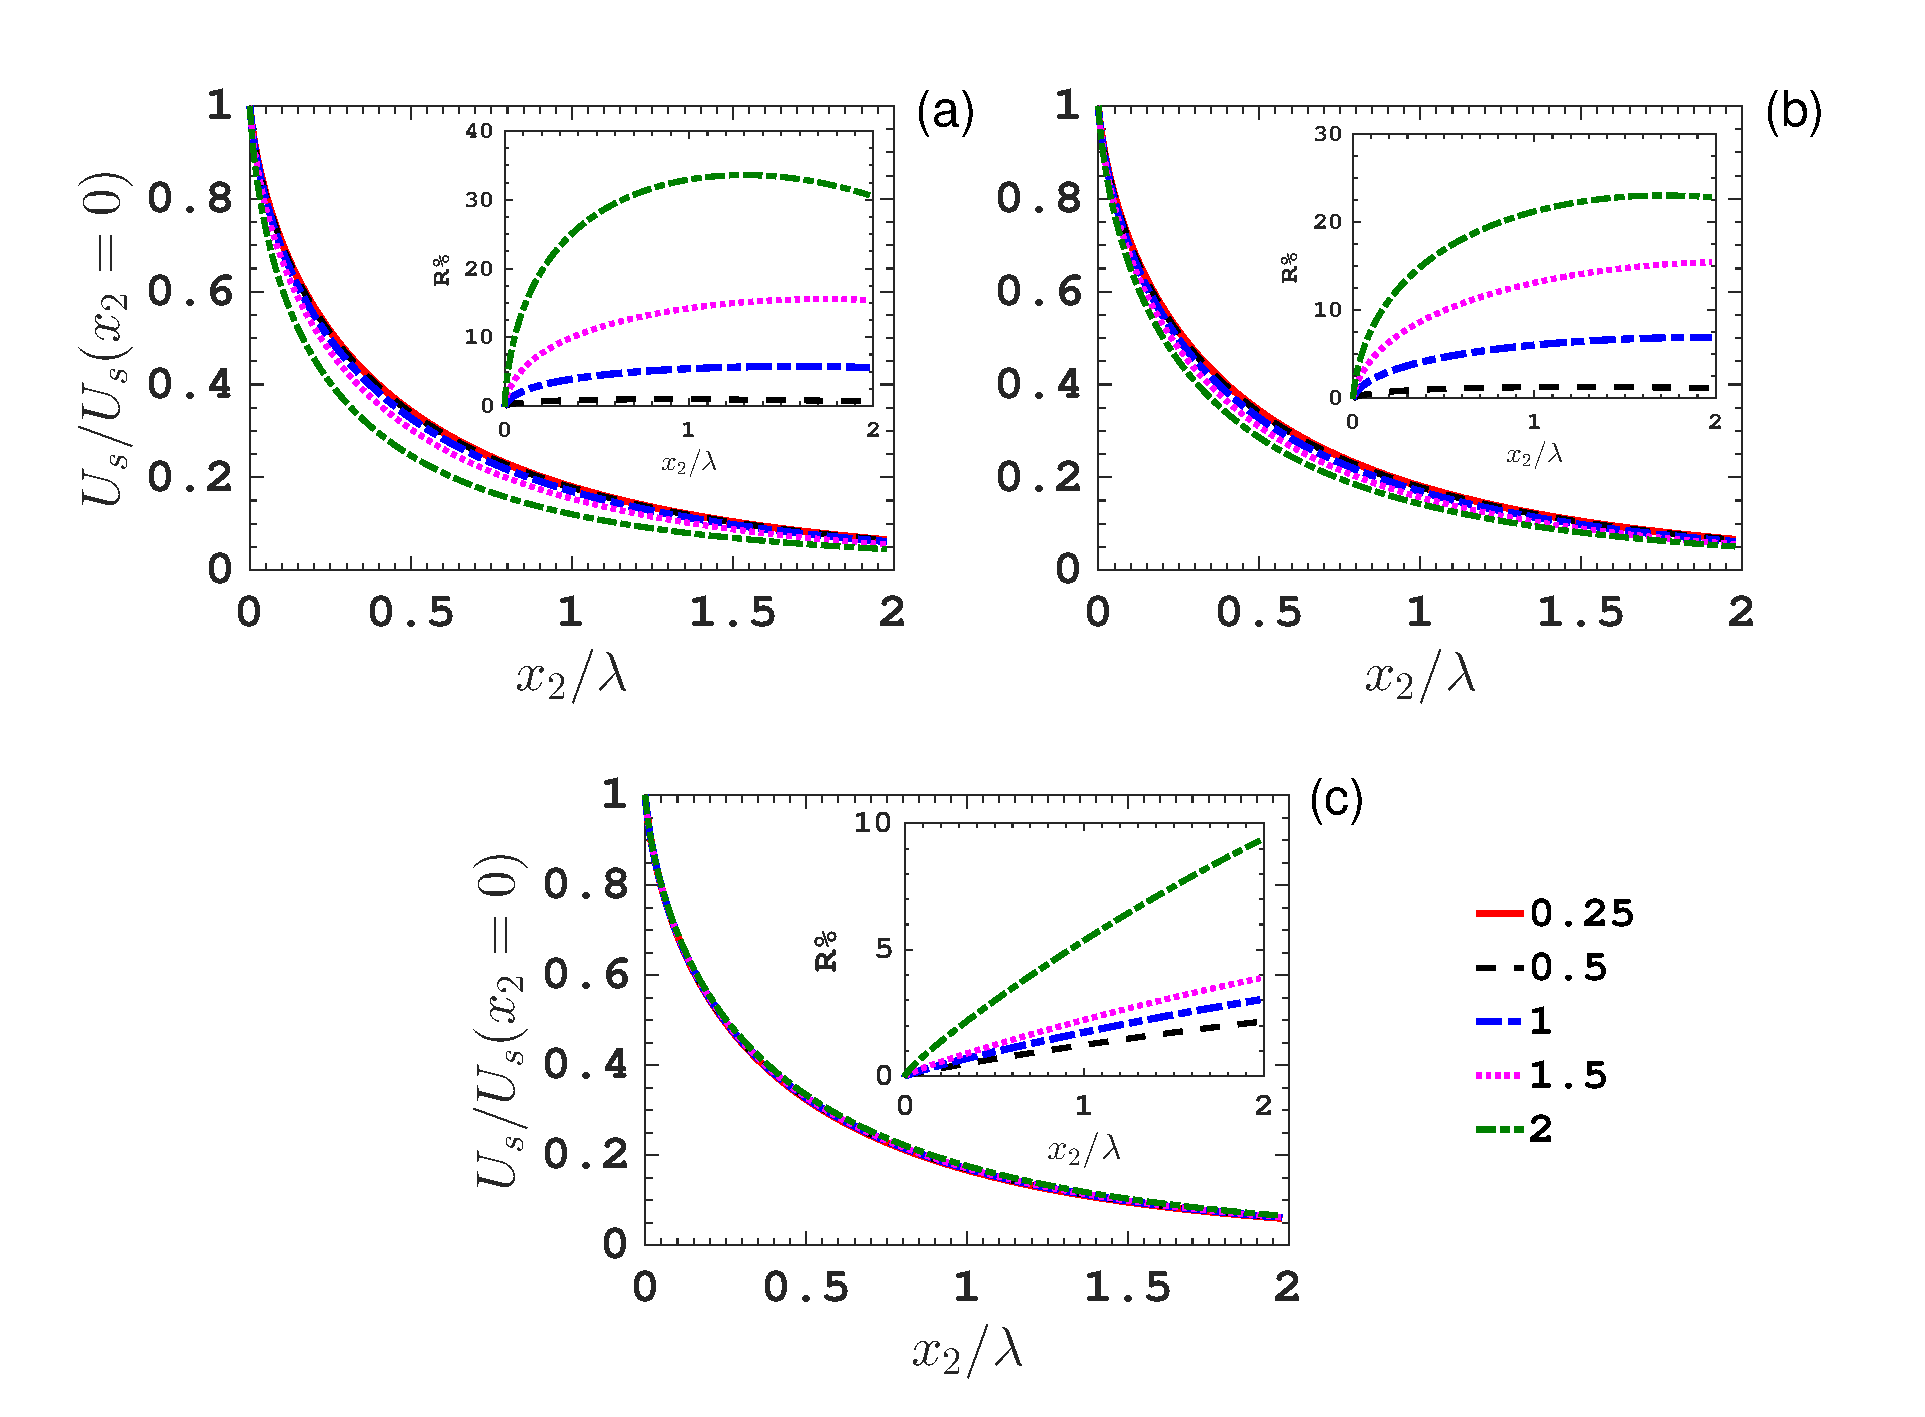
\includegraphics[width=1\textwidth]{SlipJump/IMG/check_CL}
	\caption{The rescaled KLF $u_s/u_s(x_2=0)$ of HS molecules when (a) $\alpha_n=0.25$, (b) $\alpha_n=0.5$, and (c) $\alpha_n=1$, when the Cercignani-Lampis BC with $\alpha_t=0.25, 0.5, 1.0, 1.5$, and 2.0 are used. Inset: the relative difference ($R\%$) of $u_s/u_s(x_2=0)$ at various TMAC, when compared to that of $\alpha_t=0.25$.   }
	\label{fig:vel_def_rescale_CL}
\end{figure}





%\begin{table}[thbp]
%	\centering
%	\caption{ Fitting coefficients of the rescaled KLF $u_s/u_s(0)$ for inverse power-law potentials with different values of the viscosity index $\omega$, when the diffuse BC is used. }
%	\label{table_rescale_coe}
%	\begin{tabular}{ccccccccccl}
%		\hline
%		$\omega$
%	& $c_{0,1}$  &   $c_{0,2}$ &   $c_{1,0}$ &   $c_{1,1}$ &   $c_{1,2}\cdot10$ &   $c_{2,0}$ &   $c_{2,1}$ &   $c_{2,2}\cdot 10^{2}$   \\
%		\hline
%		%%	\rowcolor[gray]{.9}
%		$0.5$
%		&  1.739 &-0.3677 & 1.628  & 1.217  & -0.4794  & -2.458 &0.1317 &0.1589 \\
%		$0.75$
%		  & 1.864   & -0.5256 &  2.113 &1.462 &-0.8429   &-2.932  &0.2245 &0.2976\\
%		$1$
%		 &  2.034  &-0.7907 & 2.820  & 1.788 &-1.5680 & -3.623 & 0.4024  &0.6003  \\
%		$1.25$
%		 &  2.275  & -1.2390 & 3.864 & 2.217  &-2.9800 & -4.648 & 0.7380   & 1.2300 \\
%		$1.5$
%	 &   2.807  & -2.5280 & 6.238& 2.821   &-8.4950 & -6.999  & 1.9310   &  4.4710 \\
%		\hline
%	\end{tabular}\par
%\end{table}



\subsubsection{Similarity in Knudsen layer function}


We study the KLF normalized by its value on the solid surface $x_2=0$, when the HS molecules are used. Results of other types of molecules are similar. For Cercignani-Lampis BC, as can be seen from Fig.~\ref{fig:vel_def_rescale_CL}, when $\alpha_n=1$, the maximum relative discrepancy for all $\alpha_t$ is less than $10\%$. When $\alpha_n$ decreases, however, the deviation of the rescaled KLF between different $\alpha_t$ increases. For instance, when $\alpha_n=0.25$, the maximum relative difference for $\alpha_t=2$ is about $30\%$, as compared with $\alpha_t=0.25$, see the inset in figure~\ref{fig:vel_def_rescale_CL}. Nevertheless, it should be noted that, for all $\alpha_n$ with $\alpha_t\le 1 $, the relative difference of the rescaled KLF is less than $7\%$.


Approximately, the KLFs is defined to have similarity if the relative difference of the rescaled KLF for different TMAC is less than $10\%$. Therefore, the KLF has the similarity when the diffuse-specular BC and the Cercignani-Lampis BC with $\alpha_n=1$ are considered, in the full range of the effective TMAC; for Cercignani-Lampis BC with other values of $\alpha_n$, the similarity is preserved when $\alpha_t\leq1$. 

%the HS molecules and the diffuse-specular BC are used.  It is found that the rescaled KLF $u_s/u_s(x_2=0)$ and their relative difference at different TMAC, when compared with that at $\alpha_M=0.2$. We notice that the rescaled KLF for $\alpha_M=0.2$ and 1 almost overlap; as shown in the inset of figure~\ref{fig:vel_def_rescale}, the maximum relative difference among all TMACs is less than $7\%$. Thus, the KLF for diffuse-specular BC possesses a good similarity between different values of TMAC.


%Under the diffuse-specular BC, the rescaled KLF can be fitted by Eq.~\eqref{eq:vel_fit}, with the fitting coefficients for different intermolecular potentials tabulated in Ref.~\cite{SU2019573}.




\subsection{Comparison with experiments}\label{sec:exp}

\begin{figure}[t]
	\begin{centering}
		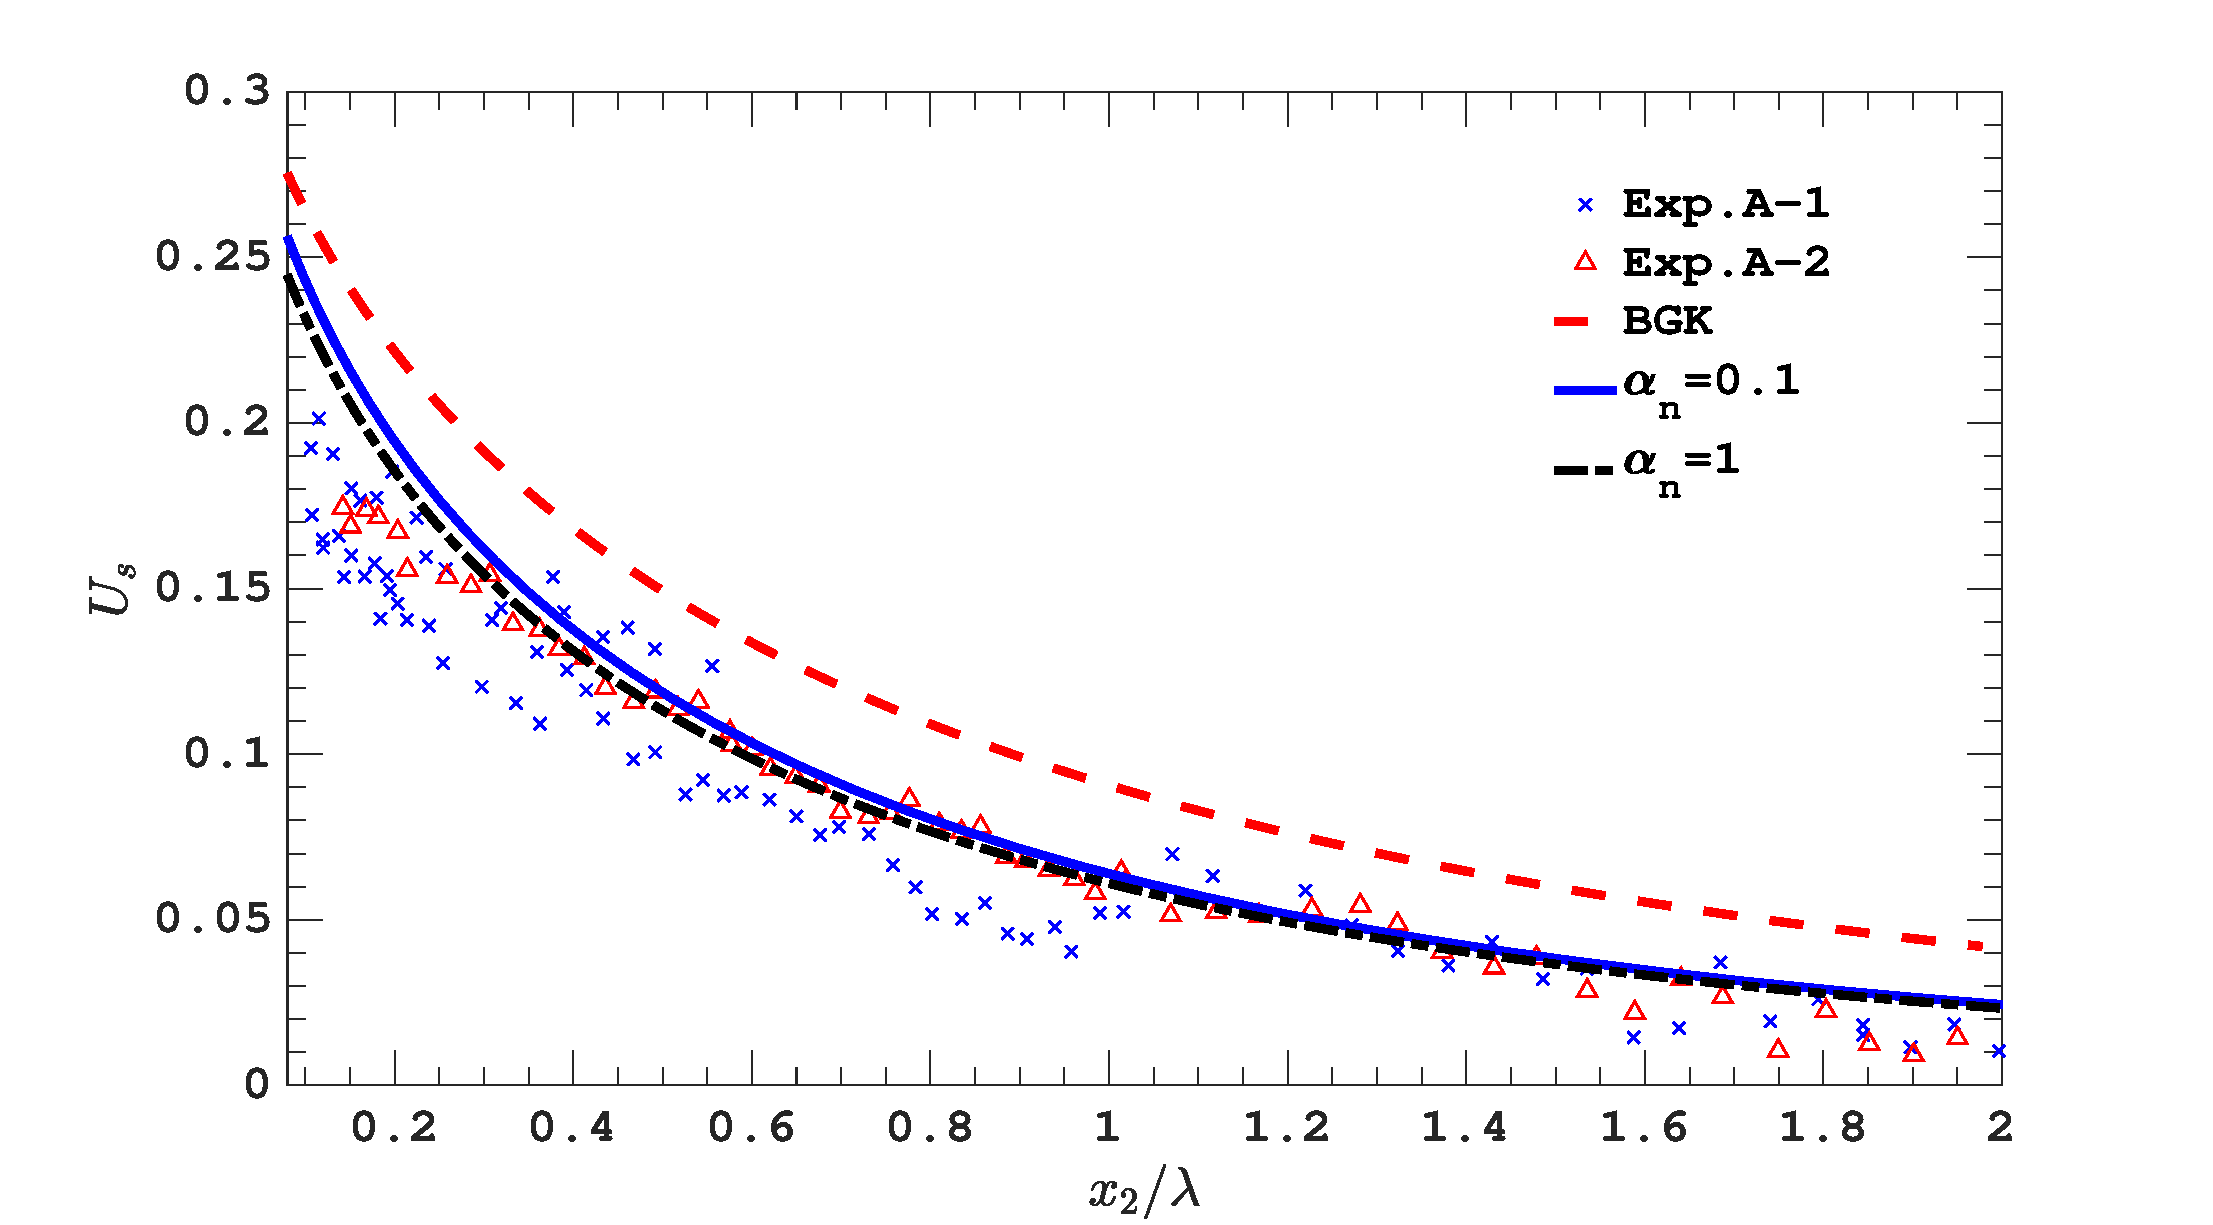
\includegraphics[width=0.8\textwidth]{SlipJump/IMG/com_exp_at088_new}
		\par\end{centering}
	\caption{ Comparisons of the KLFs between the experiments and the LBE solution with $\alpha_t=0.88$, when the air molecules of $\omega=0.75$ and various $a_n$ are applied. Exp.~A-1 and Exp.~A-2 were measured by Reynolds et al.~\cite{reynolds1974velocity}. The diffuse-specular BC with $\alpha_M=0.88$ is used in the BGK model. }
	\label{fig:com_exp}
\end{figure}


Reynolds et al. measured the VSC and KLF for air passing along the surface of a highly polished aluminum plate~\cite{reynolds1974velocity}, and found that the KLF is different from the results predicted by the BGK model. Loyalka pointed out that such discrepancy is due to the deficiency of BGK model, where the collision frequency does not depend on the molecular velocity; by using a kinetic model with a variable collision frequency, a reasonable agreement of the velocity profile with the experimental data was observed~\cite{loyalka1975velocity}. Given the apparent deficiency of kinetic models, results from the LBE of HS molecules were also compared with the experimental data~\cite{ohwada1989numerical}. However, all the previous works were based on the HS gas with an viscosity index of $\omega=0.5$, while air has an effective viscosity index of 0.75 at room temperature. Moreover, the TMAC used in numerical simulations was unity, which results in a VSC of about one, while the measured TMAC has an average value of $\sigma_P=1.1$ (which has been adjusted by multiplying a factor of $\sqrt{\pi}/2$).

\index{Knudsen layer function!Couette}

We explain the experimental data using the LBE solutions for the inverse power-law potential with $\omega=0.75$. Although air is a mixture of oxygen and nitrogen, we treat it as a single-species monatomic gas, since (i) the molecular masses of oxygen and nitrogen are close to each other and (ii) for isothermal flow the VSC is insensitive to the internal structure of gas molecules~\cite{LeiJFM2015,Loyalka1979Polyatomic}. 



%One possible reason responsible to the wrong prediction of the VSC by the LBE is that, the effective TMAC is not exactly equal to 1, due to the unavoidable roughness of the boundary surface. By averaging the results from nine separate surveys, an average VSC of $1.24$ with a range from 1.14 to 1.36 is obtained in the measurements.

Figure~\ref{fig:com_exp} shows the KLF obtained from the LBE with $\alpha_t=0.95$, and $\alpha_n=0.1$ and 1 under the Cercignani-Lampis BC, as well as the experimental data. The result from the BGK equation is also included for comparison. We use the value of TMAC $\alpha=0.95$, as our numerical calculation in the previous section suggests that the predicted VSC from the LBE agrees well with the experimental value of 1.1~\cite{reynolds1974velocity}. It is found that the KLF changes slightly under different $\alpha_n$, and the results of $\alpha_n=1$ seems better than the others in the agreement with the experimental data, while the solution of the BGK equation has a visible deviation from the experimental results. Note that when using the diffuse-specular BC, similar results can also be obtained for $\alpha_M=0.95$.



\begin{figure}[t]\label{com_air}
	\begin{centering}
		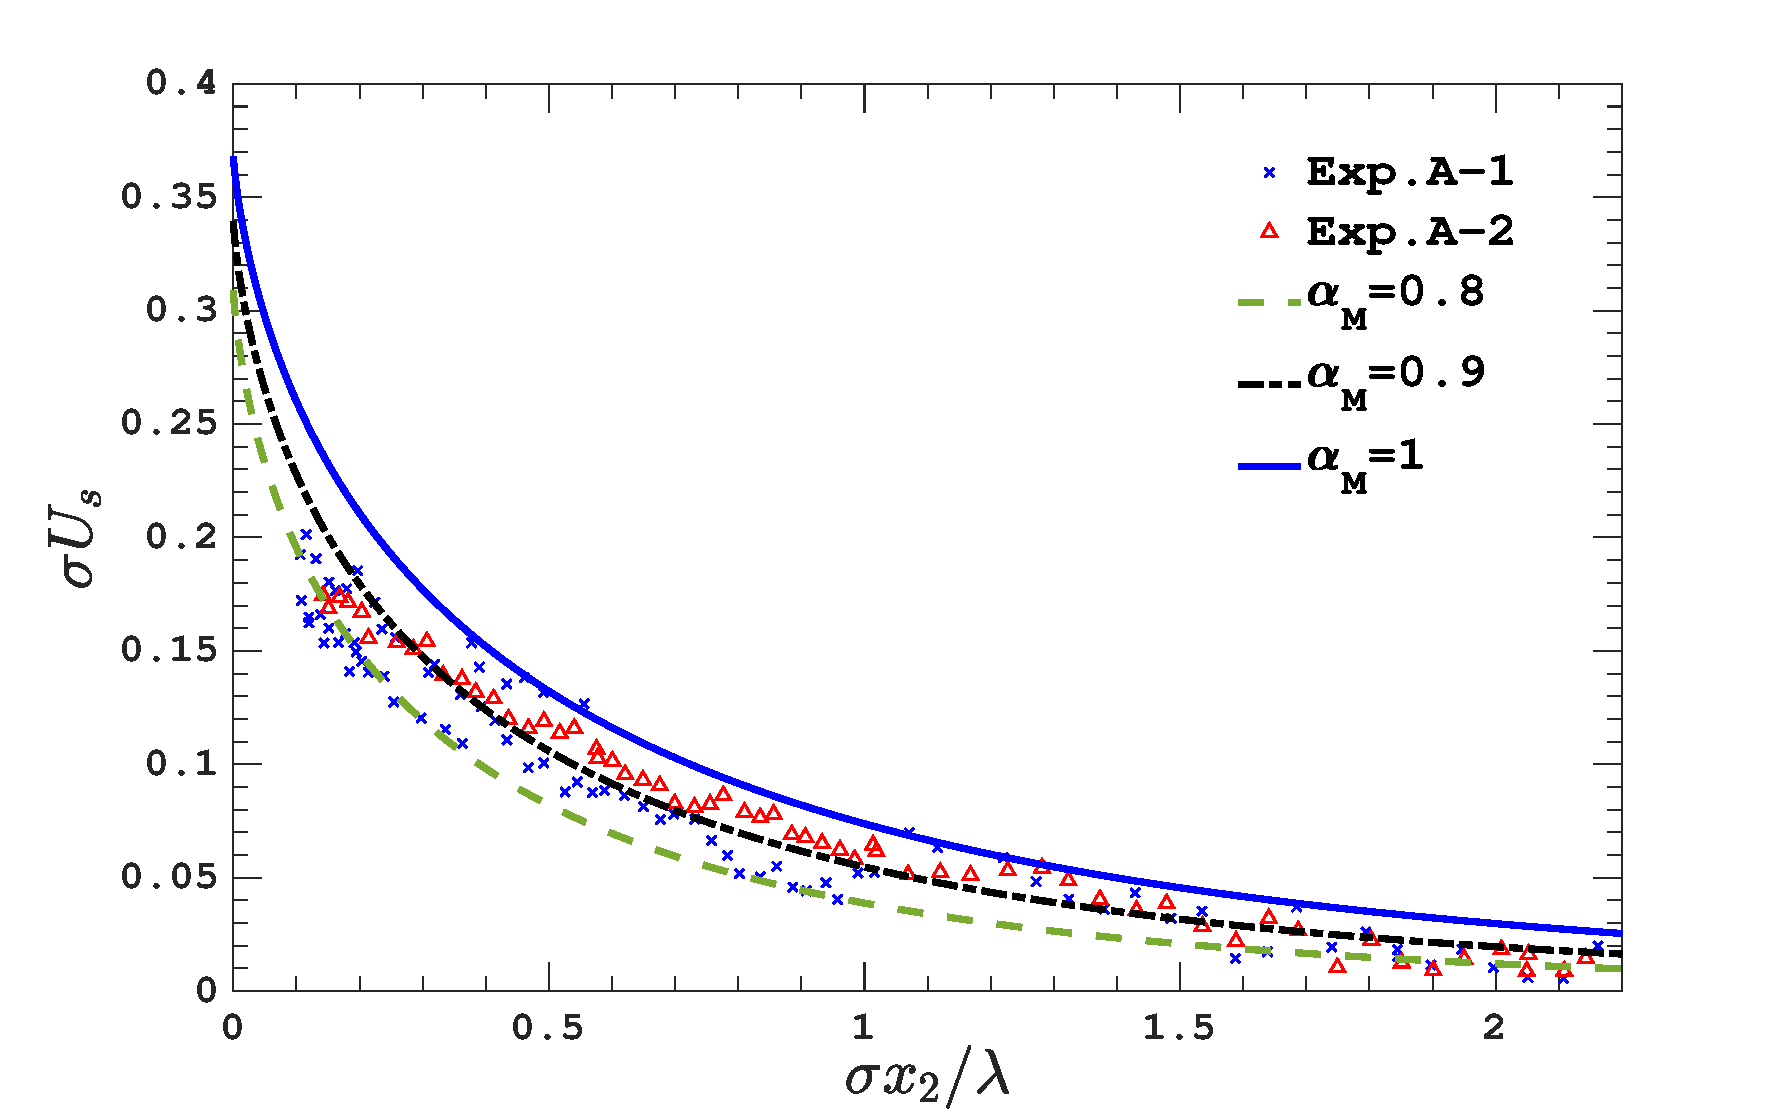
\includegraphics[width=0.7\textwidth]{SlipJump/IMG/rescale_KLF_new}
		\par\end{centering}
	\caption{ Comparisons of the KLF between the experiments and the LBE solution with $\alpha_M=0.8,~0.9$ and 1, when the air molecules with $\omega=0.75$ are used. LBE results are scaled by a factor $\sigma=\sigma_{P,Exp}/\sigma_P(\alpha_M)$, where $\sigma_{P,Exp}=1.1$ is the average VSC from the experiments~\cite{reynolds1974velocity}. }
	\label{fig:com_exp_air}
\end{figure}

We note that the KLF from the experiments are scattered, which is inconsistent with the theoretical analysis that the normalized velocity near the solid surface should be independent of the MFP and shear gradient. Reynolds et al.~\cite{reynolds1974velocity} argued that the most possible reason was the inaccurate determination of the MFP. Therefore, intuitively, in order to interpret the experimental results, one should take this factor into account. To this end, we first assume the actual TMAC for the interaction of air with the polished aluminum plate is $\alpha_M$ in the diffuse-specular BC. Then we calculate the VSC $\sigma_P(\alpha_M)$ from the LBE. If $\sigma_{P,Exp}<\sigma_P(\alpha_M)$, the MFP in the experiment has been overestimated due to the inaccurate  measuring of the gas pressure. Therefore, the value of the KLF from the experiment~\cite{reynolds1974velocity} should be multiplied by  $1/\sigma=\sigma_P(\alpha_M)/\sigma_{P,Exp}$, while the width of the KLF should be stretched by a factor of $1/\sigma$. In the numerical simulation, various values of $\alpha_M$ are attempted, until good agreement between the results of experiment and numerical simulation are achieved.   





To show all the results in one figure, however, the KLF $u_s(x_2)$ obtained from the numerical simulation of the LBE has been rescaled to $\sigma{u_s}(\sigma{}x_2)$. Comparisons between the numerical and experimental results are depicted in Fig.~\ref{fig:com_exp_air}. It is seen that, when the TMAC varies from 0.8 to 1, the results of LBE can cover almost all the experimental data. In other words, the TMAC of the aluminum plate used in the air experiments is most likely $0.9\pm0.1$. If the TMAC is 0.9, we have $\sigma=0.9$, this means that the MFP in the experiment is overestimated by $10\%$, which seems reasonable due to the accuracy of the micro-manometers at that time.


\section{Planar Fourier flows}\label{Fourier_lin_FSM}
\index{Fourier flow}


\begin{figure}[tp]
	\centering
	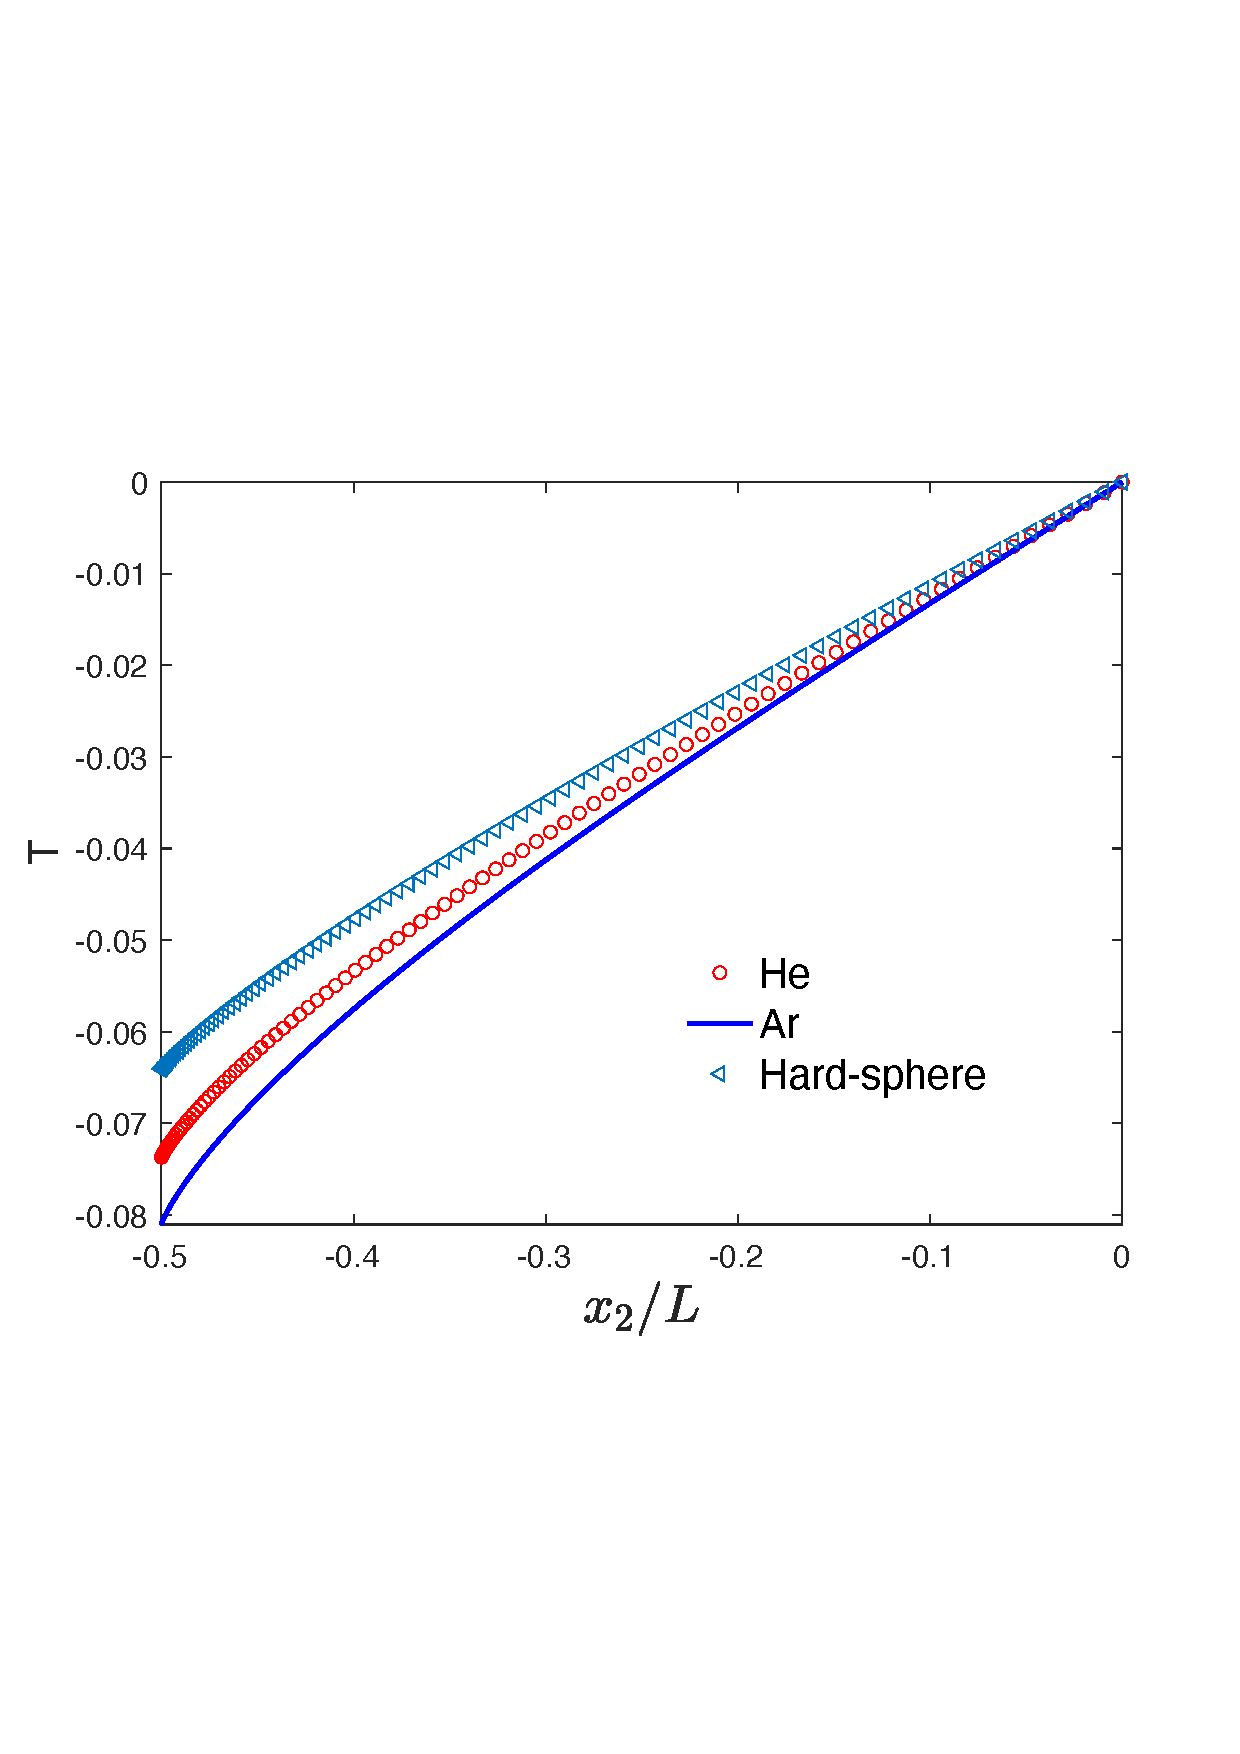
\includegraphics[width=0.46\columnwidth]{LinearizedBol/IMG/FourierDelta01T}
	\hskip 0.5cm
	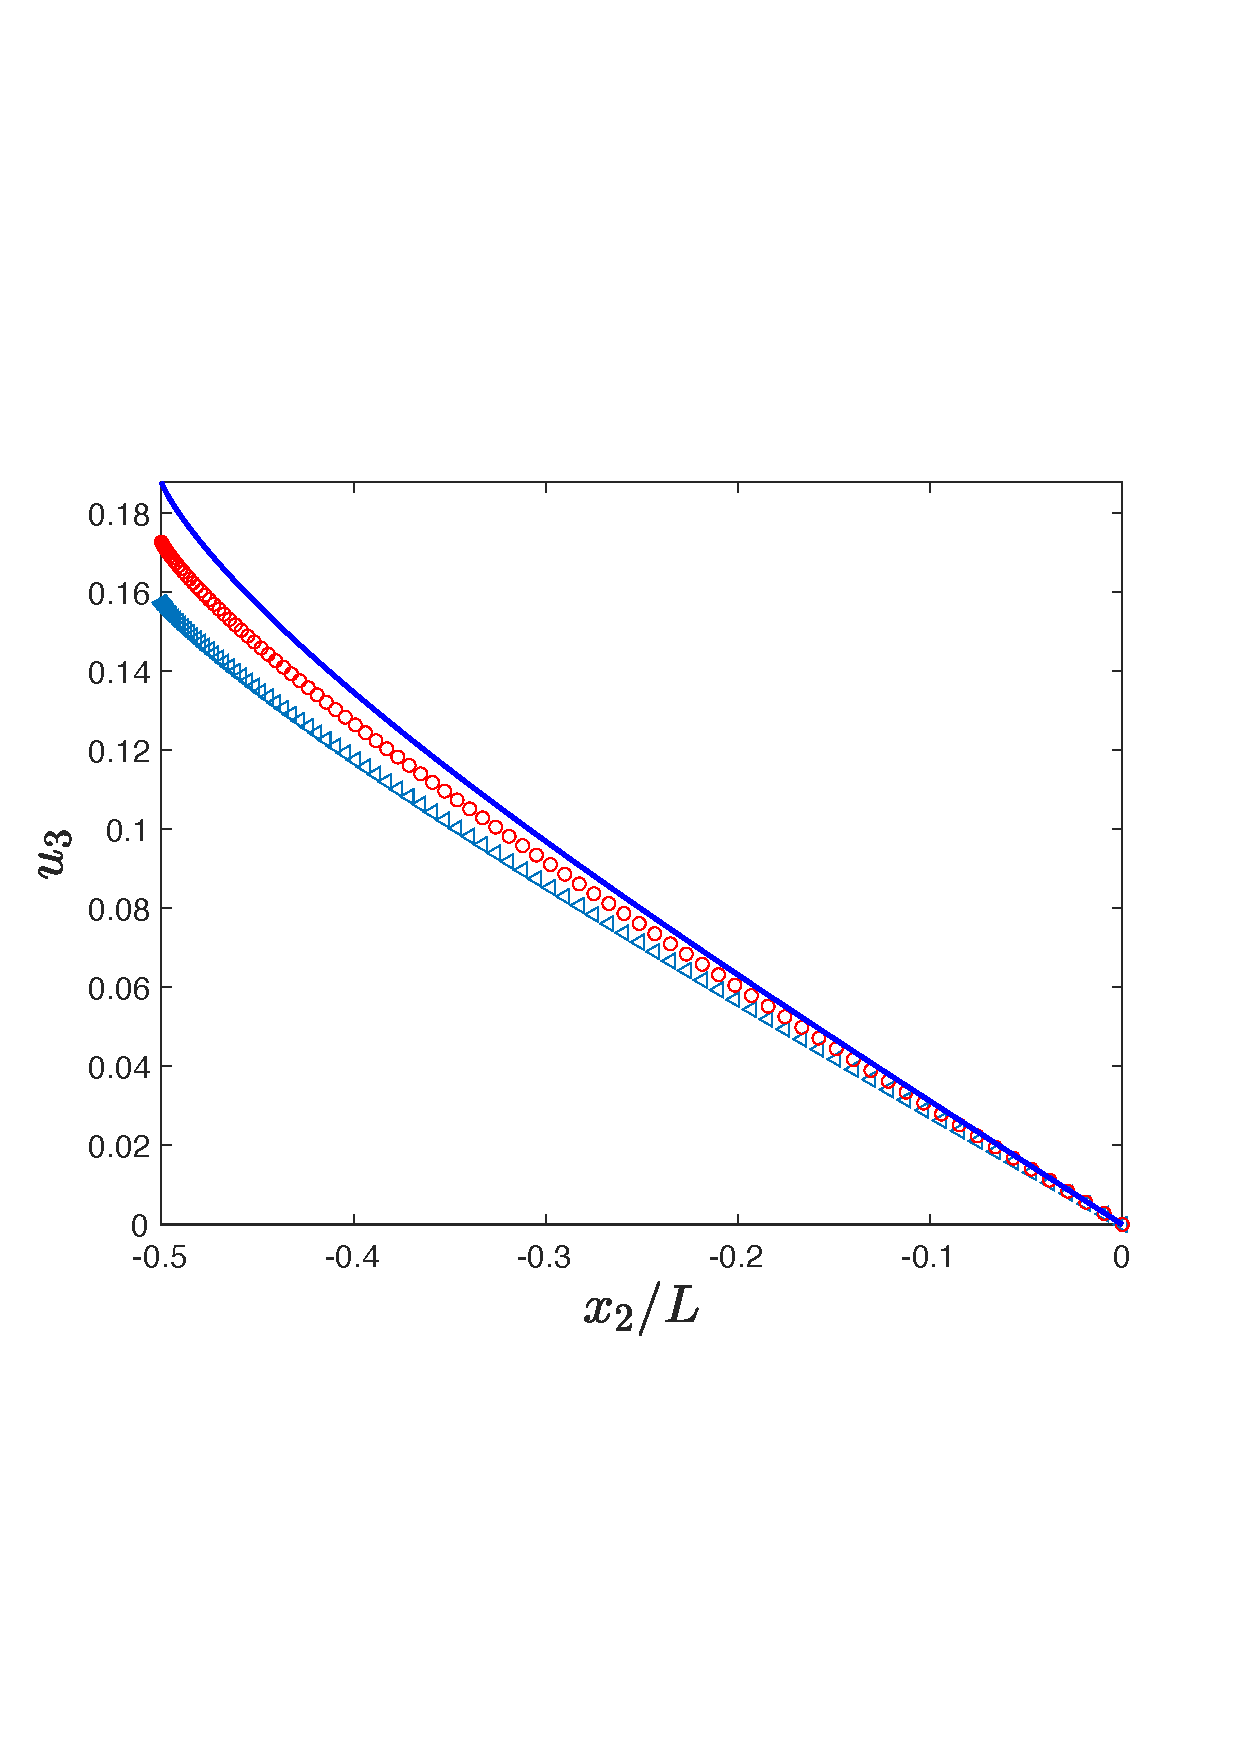
\includegraphics[width=0.46\columnwidth]{LinearizedBol/IMG/LJCouetteDelta01V}
	\caption{
		Normalized density (velocity) in the planar Fourier (Couette) flow~\cite{wuPoF2015}, obtained from the LBE with the collision kernel directly calculated from the Lennard-Jones potential. Results from the HS gas are shown for comparison.  The rarefaction parameter is $\delta_{rp}=0.1$. 
	}
	\label{Fourier_lin}
\end{figure}

Consider the Fourier heat conduction between two plates located at $x_2=-0.5$ and $x_2=0.5$, where the temperature is $T_0-\Delta{T}/2$ and  $T_0+\Delta{T}/2$, respectively. The temperature difference $\Delta{T}$ is negligible compared to $T_0$, so that the Boltzmann equation~\eqref{Boltzmann_dimensionless} is linearized to Eq.~\eqref{Chapter1_Boltzmann_lin} by choosing as $\beta=\Delta{T}/T_0$. Assuming diffuse BC, the VDF reflected from the wall reads
\begin{equation}\label{Fourier_boundarycondition}
h= \left[ 1-\frac{v^2}{2}-2\sqrt{\pi}\int_{v_2<0} v_2h\left(v,x_2=-0.5\right)dv\right] f_{eq}, 
\end{equation}
while at $x_2=0$, the symmetry leads to $h(v_1,v_2,v_3)=-h(v_1,-v_2,v_3)$.

%The spatial region $-1/2\le{x_2}\le0$ is discretized by 100 non-uniform grid points, with most of the grid points located near the wall, see Eq.~\eqref{spatial_d}. The three-dimensional molecular velocity domain $[-6,6]^3$ is discretized by $32\times128\times32$ grid points, and the number of frequency components is $32\times48\times32$.  

%The iterative scheme ${v_2}{\partial h^{(k+1)}}/{\partial x_2}+\nu_{eq}(v)h^{(k+1)}=\mathcal{L}^+(h^{(k)})$ is used, and the iterations are terminated when the maximum relative difference in the density $n=\int hdv$, temperature $T=2\int hv^2dv/3-n$, and heat flux $q_2=\int hv^2v_2dv$ between two consecutive steps is less than $10^{-5}$. 

Figure~\ref{Fourier_lin} shows the density when $\delta_{rp}=0.1$ and $T_0=300$~K; the temperature has similar behavior (not shown). The influence of intermolecular potential is clearly seen, e.g., the density of Xe at the wall is 40\% larger than that of the HS gas. As $\delta_{rp}$ increases, the difference decreases, which eventually disappears in near-continuum flow.  Interestingly, differences in heat flux between various gases is small over the whole range of rarefaction parameter.



\section{Thermal transpiration}\label{poiseuille_dis}
\index{thermal transpiration}



%It has found applications in many engineering problems, including the Crookes radiometer~\cite{crookes1874xv}, the Knudsen compressor that pumps the gas without any moving mechanical part~\citep{vargo1999knudsen,gupta2008thermal}, the capacitance diaphragm gauge where the effects of thermal transpiration should be subtracted for accurate measurement of low gas pressures~\citep{Sentina1999,Daude2014Vacuum}, gas mixture separation~\citep{Takata2007EJMB}, and the Leidenfrost ratchet which rectifies the vapor flow in the boundary layer~\citep{wurger2011leidenfrost}. Thermal transpiration arises when the Knudsen number becomes appreciable in micro/nano-devices and/or low-pressure environments.


Thermal transpiration, where the gas moves towards a hotter region even in the absence of a pressure gradient, is one of the fundamental problems in RGD~\citep{Reynolds1879,Maxwell1879vii}. The gas pressure is maintained constant, while the wall temperature varies linearly in the $x_3$ direction as
\begin{equation}
T=T_0\left(1+\beta_T\frac{x_3}{L}\right), \quad
\beta_T=\frac{L}{T_0}\frac{dT}{dx_3},
\end{equation} 
where the dimensionless temperature gradient $\beta_T$ is very small. The Boltzmann equation can be linearized around the equilibrium state, when $h$ in Eq.~\eqref{Chapter_lin_VDF} is replaced by $h+x_3f_{eq}({v}^2-\frac{5}{2})$, resulting 
\begin{equation}\label{thermal_tube}
v_1\frac{\partial h}{\partial x_1}+v_2\frac{\partial h}{\partial x_2}=\mathcal{L}^+(h)-\nu_{eq}{h}-{v_3}\left({v}^2-\frac{5}{2}\right)f_{eq}.
\end{equation}
The MFR and HFR are expressed as
\begin{equation}\label{normalized_MFR_thermal}  
\begin{aligned}[b]
\dot{M}&=\frac{2p_0S}{v_m}\beta_TG_T, \quad  G_T=\frac{1}{A}\iiint {v_3h}dx_1dx_2d\bm{v}, \\
\dot{E}&=-p_0v_mS\beta_T{}Q_T, \quad   Q_T=-\frac{1}{A}\iiint {\left({v}^2-\frac{5}{2}\right)v_3}hdx_1dx_2d\bm{v}.
\end{aligned}
\end{equation}





%
%
%\begin{table}[t]
%	\centering
%	\caption{MFR and HFR in the thermal transpiration of HS gas through a rectangular channel~\cite{Wu2013PhDthesis}. Note that $\text{Kn}=5\pi{}k'/16$.} \label{table_thermal_2d_compare} 
%		\centering
%		\begin{tabular}{cccccccccccc}
%			\hline
%			&  \multicolumn{4}{c}{$A=1$} & \multicolumn{4}{c}
%			{$A=2$}        \\  
%			&  \multicolumn{2}{c}{FSM} & \multicolumn{2}{c}{Doi~\cite{Doi2010}}  
%			&  \multicolumn{2}{c}{FSM}    &  \multicolumn{2}{c}{Doi~\cite{Doi2010}}  
%			\\  \hline 
%			$k'$ & $G_T$ & $Q_T$ & $G_T$ & $Q_T$ & $G_T$ & $Q_T$ & $G_T$ & $Q_T$ \\  
%			0.1    & 0.0450 & 0.1759  & 0.045  & 0.176   & 0.0479 & 0.1842 & 0.048  & 0.185  \\  
%		%	0.2    & 0.0719 & 0.2936  & 0.072  & 0.294   & 0.0793	& 0.3199 & 0.079  & 0.320  \\  
%			0.3    & 0.0891 & 0.3748  & 0.089  & 0.375   & 0.1014 & 0.4205 & 0.101  & 0.421  \\ 
%		%	0.4    & 0.1012 & 0.4341  & 0.102  & 0.434   & 0.1176	& 0.4976 & 0.118  & 0.498  \\  
%			0.5    & 0.1103 & 0.4794  & 0.110  & 0.479   & 0.1302 & 0.5587 & 0.130  & 0.560  \\
%		%	0.6    & 0.1174 & 0.5153  & 0.118  & 0.514   & 0.1403 & 0.6085 & 0.140  & 0.609  \\
%			0.8    & 0.1279 & 0.5690  & 0.128  & 0.568   & 0.1556 & 0.6852 & 0.155  & 0.686  \\
%			1      & 0.1356 & 0.6077  & 0.136  & 0.606   & 0.1668	& 0.7433 & 0.167  & 0.743  \\
%		%	2      & 0.1560 & 0.7098  & 0.156  & 0.708   & 0.1980 & 0.9003 & 0.198  & 0.900  \\  
%			3      & 0.1658 & 0.7571  & 0.166  & 0.756   & 0.2135 & 0.9762 & 0.214  & 0.976  \\
%		%	4      & 0.1719 & 0.7856  & 0.172  & 0.784   & 0.2233 & 1.0229 & 0.223  & 1.023  \\
%			5      & 0.1761 & 0.8052  & 0.176  & 0.804   & 0.2303 & 1.0553 & 0.230  & 1.055  \\
%		%	6      & 0.1793 & 0.8197  & 0.179  & 0.818   & 0.2355 & 1.0795 & 0.236  & 1.079  \\
%			8      & 0.1839 & 0.8399  & 0.184  & 0.839   & 0.2431 & 1.1136 & 0.243  & 1.113  \\
%			10     & 0.1870 & 0.8536  & 0.187  & 0.852   & 0.2484 & 1.1370 & 0.248  & 1.136  \\
%			20     & 0.1950 & 0.8867  & -      &-        & 0.2618 & 1.1942 & -      & -      \\
%			50     & 0.2017 & 0.9138  & -      &-        & 0.2736 & 1.2420 & -      & -      \\
%			$10^2$ & 0.2048 & 0.9258  & -      &-        & 0.2792 & 1.2636 & -      & -      \\
%			$10^3$ & 0.2089 & 0.9406  & -      &-        & 0.2866 & 1.2909 & -      & -      \\   
%			$10^4$ & 0.2095 & 0.9430  & -      &-        & 0.2878 & 1.2954 & -      & -      \\   
%			$\infty$\footnote{Data in columns 4, 5, 8, and 9 are obtained from Eq.~\eqref{Mass_flow_rate_fm}.} & 0.2097 & 0.9436  & 0.2097 & 0.9436  & 0.2881 & 1.2965 & 0.2881 & 1.2965 \\
%			\hline
%		\end{tabular}\par
%		\vspace{-0.75\skip\footins}
%		\renewcommand{\footnoterule}{}
%\end{table}


\begin{figure}[t]
	\centering
	{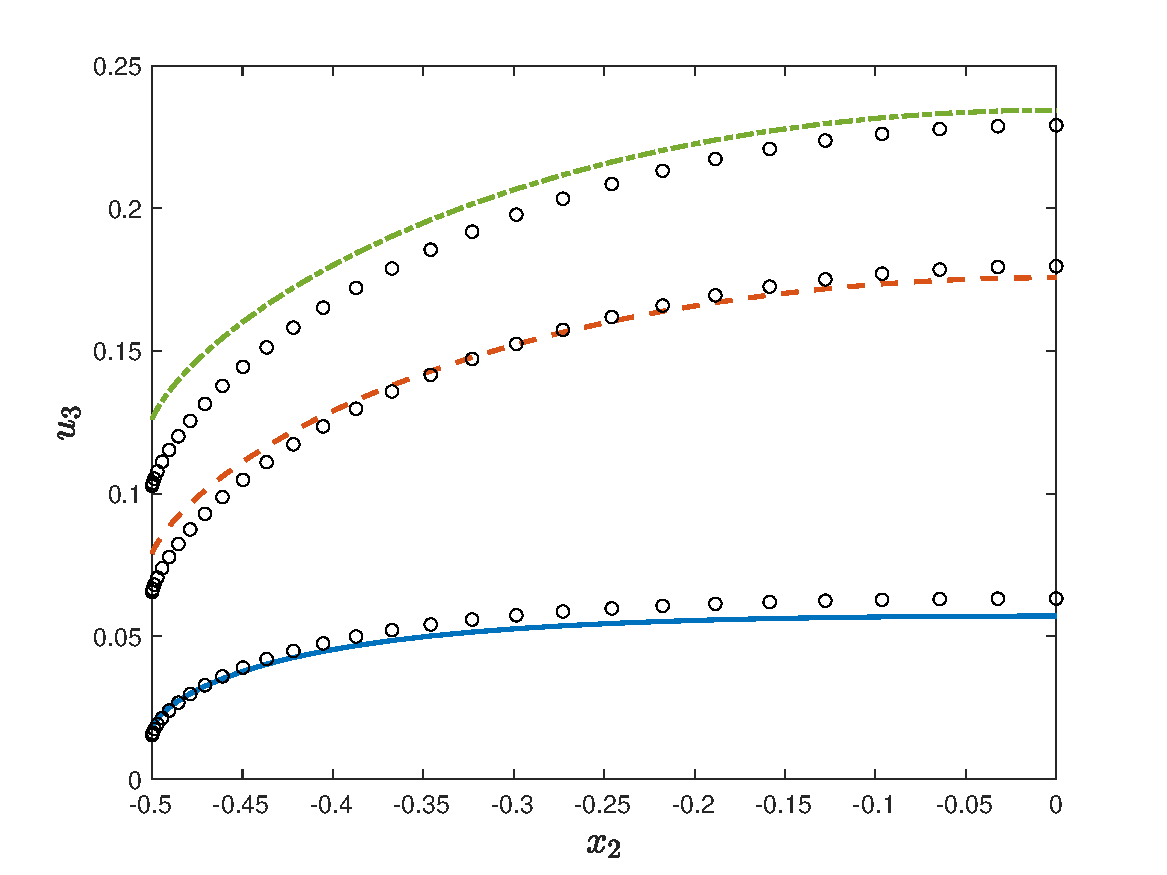
\includegraphics[scale=0.45]{LinearizedBol/IMG/Transpiration_1D.pdf}} 	{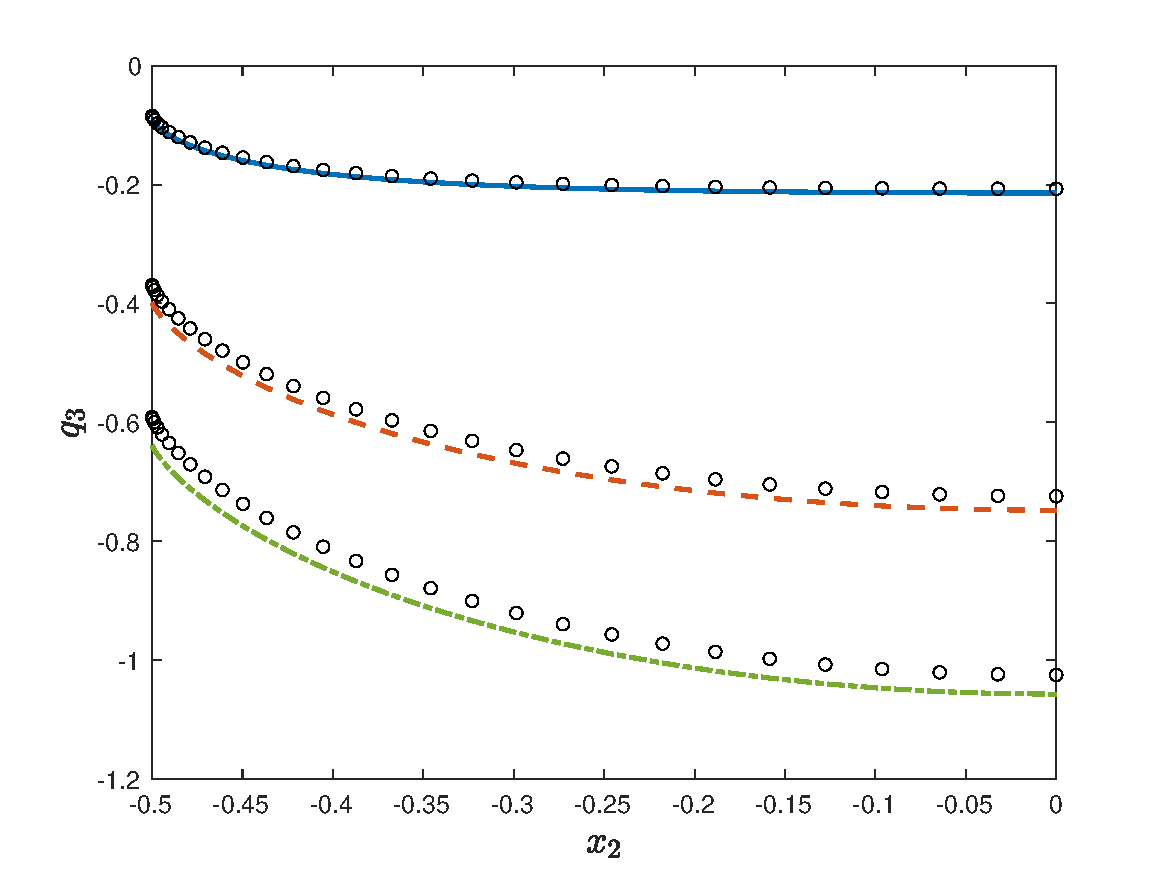
\includegraphics[scale=0.45]{LinearizedBol/IMG/Transpiration_1D2.pdf}}
	\caption{
		Profiles of velocity and heat flux in the thermal transpiration between two parallel plates. Solid, dashed, dash-dotted lines are the results of HS gas, when $\text{Kn}=0.1$, 0.5, and 1, respectively, while circles are the corresponding results of Maxwell gas.
	} 
	\label{Transpiration_massheat}
\end{figure}


Typical profiles of the velocity and heat flux are shown in Fig.~\ref{Transpiration_massheat}, whose magnitudes increase with the Knudsen number. Again, it is observed that although the Knudsen number is the same, different intermolecular potential (viscosity index) has different macroscopic profiles. \index{viscosity index}



For the rectangular cross-section, the mass flow rate is $G_T=\mathcal{M}/{2}$ and the heat flow rate in the free-molecular flow regime~\cite{loyalka1976} is $G_T={9}\mathcal{M}/4$, where $\mathcal{M}$ is given by Eq.~\eqref{Mass_flow_rate_fm}. 

%The comparison in MFR and HFR with Doi's results are shown in Table~\ref{table_thermal_2d_compare}, where good agreements can be found.


%
%\leir{effect shear viscosity and thermal conductivity}
%\newpage

\section{Poiseuille flow }
\label{FSM_linear_Poiseuille}
\index{Poiseuille flow}

Consider an infinite long channel of a cross-section area $S$ located in the $x_1x_2$ plane. The gas inside is subject to a uniform pressure gradient in the $x_3$ direction:
\begin{equation}
p=p_0\left(1+\beta_p{}\frac{x_3}{L}\right), \quad
\beta_p=\frac{L}{p_0}\frac{dp}{dx_3},
\end{equation}
and the dimensionless pressure gradient $\beta_p$ is very small. Both the wall and gas temperature are kept at $T_0$. The mass flow rate (MFR) and heat flow rate (HFR), are defined as
\begin{equation}\label{MFR_HFR}
\begin{aligned}[b]
\dot{M}=n_0m\iint {}u_3(x_1,x_2)dx_1dx_2,\quad
\dot{E}=\iint       q_3(x_1,x_2)dx_1dx_2.
\end{aligned}
\end{equation}

The Boltzmann equation can be linearized around the equilibrium state, when $h$ in Eq.~\eqref{Chapter_lin_VDF} is replaced by $h+x_3f_{eq}$, resulting 
\begin{equation}\label{poiseuille_tube}
v_1\frac{\partial h}{\partial x_1}+v_2\frac{\partial h}{\partial x_2}=\mathcal{L}^+(h)-\nu_{eq}{h}-{v_3}f_{eq}.
\end{equation}
Note that here the macroscopic variables and VDF have been normalized, so that the MFT and HFR are expressed as
\begin{equation}\label{normalized_MFR}
\begin{aligned}[b]
\dot{M}=-\frac{2p_0S}{v_m}\beta_pG_P,\quad
\dot{E}=p_0v_mS\beta_p{}Q_p,
\end{aligned}
\end{equation}
with the normalized MFT and HFR
\begin{equation}
\begin{aligned}[b]
G_P=-\frac{1}{A}\iint {u_3}dx_1dx_2\equiv -\frac{1}{A}\iiint {v_3h}dx_1dx_2d\bm{v}, \\  
Q_p=\frac{1}{A}\iint {q_3}dx_1dx_2\equiv
\frac{1}{A}\iiint {\left({v}^2-\frac{5}{2}\right)v_3}hdx_1dx_2d\bm{v}, 
\end{aligned}
\end{equation}
where $A=S/L^2$. 




\subsubsection{Poiseuille flow between parallel plates}

Consider the Poiseuille flow between two plates located at $x_2=\pm1/2$. The spatial region is divided into $N_s=50$ non-uniform cells, as
\begin{equation}\label{spatial_d}
x=(10-15s+6s^2)s^3, 
\end{equation}
with $s=(0,1,\cdots,N_s)/N_s$. Such a non-uniform discretization has refined grids in the vicinity of solid walls, hence helps to capture the Knudsen layer structure.
Because of symmetry, we only consider the half spatial region $-1/2\le{}x_2\le0$ with the specular-reflection BC being imposed at $x_2=0$. The diffuse BC is adopted at the wall: 
\begin{equation}
h\left(x_2=-{1}/{2},v_2>0\right)=0.
\end{equation}

The maximum molecular velocity is $L_v=6$. Because of the symmetry and smoothness of the VDF in $v_1(>0)$ and $v_3(>0)$ directions, $12\times12$ uniform grids are used. In the discretization of $v_2$, $N_v=64$ nonuniform velocity grids~\eqref{nonuniform_v} with $\imath=3$ are used to resolve the over-concentration of VDF at large Knudsen numbers. \index{non-uniform velocity discretization}
The number of frequency components in the $\xi_1$ and $\xi_3$ directions are 24. Although we use $N_v$ nonuniform velocity grids in $v_2$ direction, the corresponding frequency domain is divided into $32$ equidistant points. In the approximation of the kernel mode~\eqref{kernel_mode2}, the Gauss-Legendre quadrature with $M=10$ is used. The Matlab code is given in Appendix~\ref{appen_Poiseuille}, where besides the CIS, the general synthetic iterative scheme~\cite{LeiJCP2017,SuArXiv2019} detailed in Chapter~\ref{chap:GSIS} is implemented to find the steady-state solution efficiently and accurately. 

%The FSM results are compared to those in Refs.~\cite{Ohwada_sone_1989,Takata2011} for a gas of HS molecules, where the absolute errors between the two methods in the mass and heat flow rates are less than $2\times10^{-4}$, demonstrating the high accuracy of FSM. 

%% , 
%\begin{equation}\label{iteration_linear}
%{\nu_{eq}}{h}^{k+1}+{v_2}\frac{\partial {h}^{k+1}}{\partial
%	{x_2}}=\mathcal{L}^+(h^k)-{v_1}f_{eq}.
%\end{equation}
%where $\partial h/\partial x_2$ is approximated by the  second-order upwind finite difference. The iteration is terminated when the MFR between two consecutive iteration step is less than $10^{-5}$

Typical profiles of the velocity and heat flux are shown in Fig.~\ref{massheat}. When $\text{Kn}=0.1$, the velocity is large. The velocity profile becomes flatter when the Knudsen number increases, due to the increased friction between gas molecules. When the Knudsen number is larger than 1, however, the velocity slip at the solid wall increases, which compensates the friction. As a result, a minimum MFR around $\text{Kn}\sim1$ appears, which is known as the Knudsen minimum. 
\index{Knudsen minimum} \index{Poiseuille flow} 
The HFR always increases with the Knudsen number. 

At large Knudsen number, the MFR and HFR are sensitive to the intermolecular potential (reflected through the viscosity index $\omega$), \index{viscosity index} even when the Knudsen number is fixed. That is, the smaller the viscosity index, the larger the mass and heat flow rates. 

\begin{figure}[t]
	\centering
	{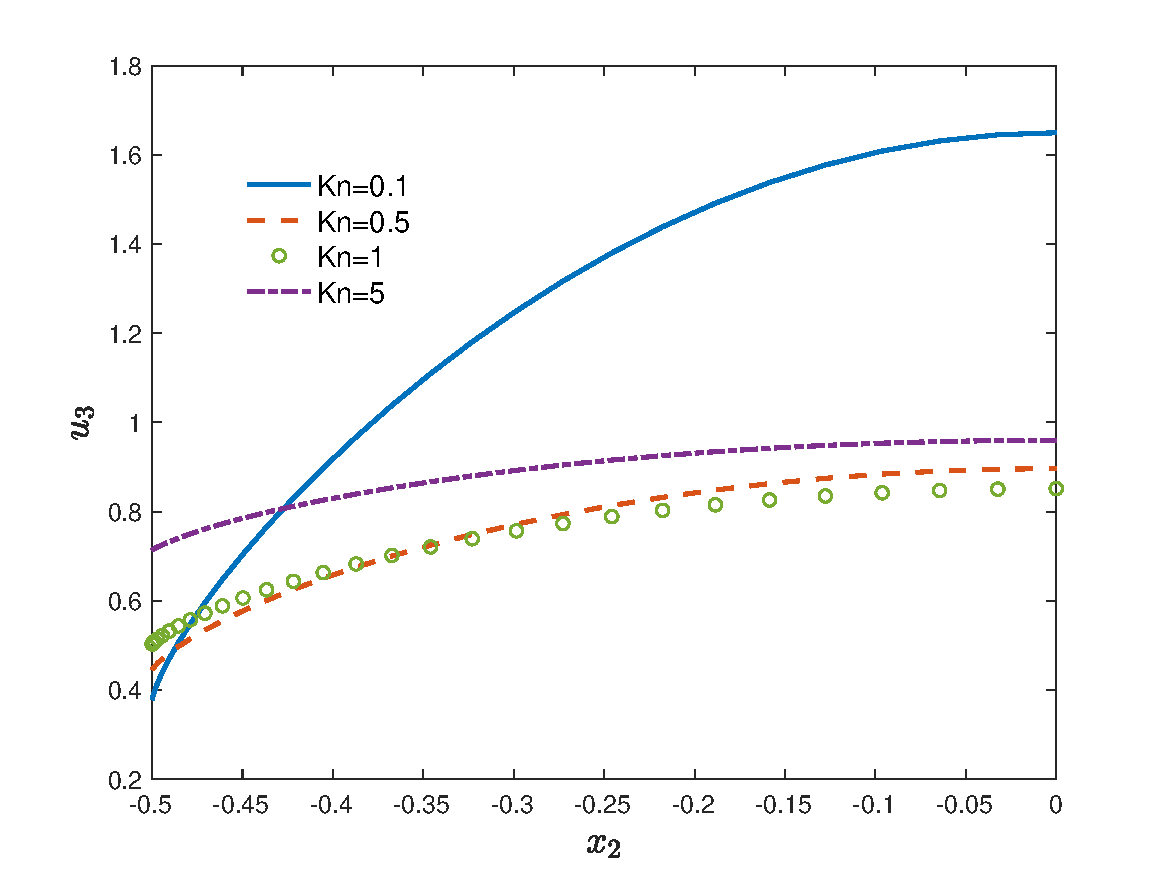
\includegraphics[scale=0.4]{LinearizedBol/IMG/Poiseuille_1D_HS.pdf}} 	{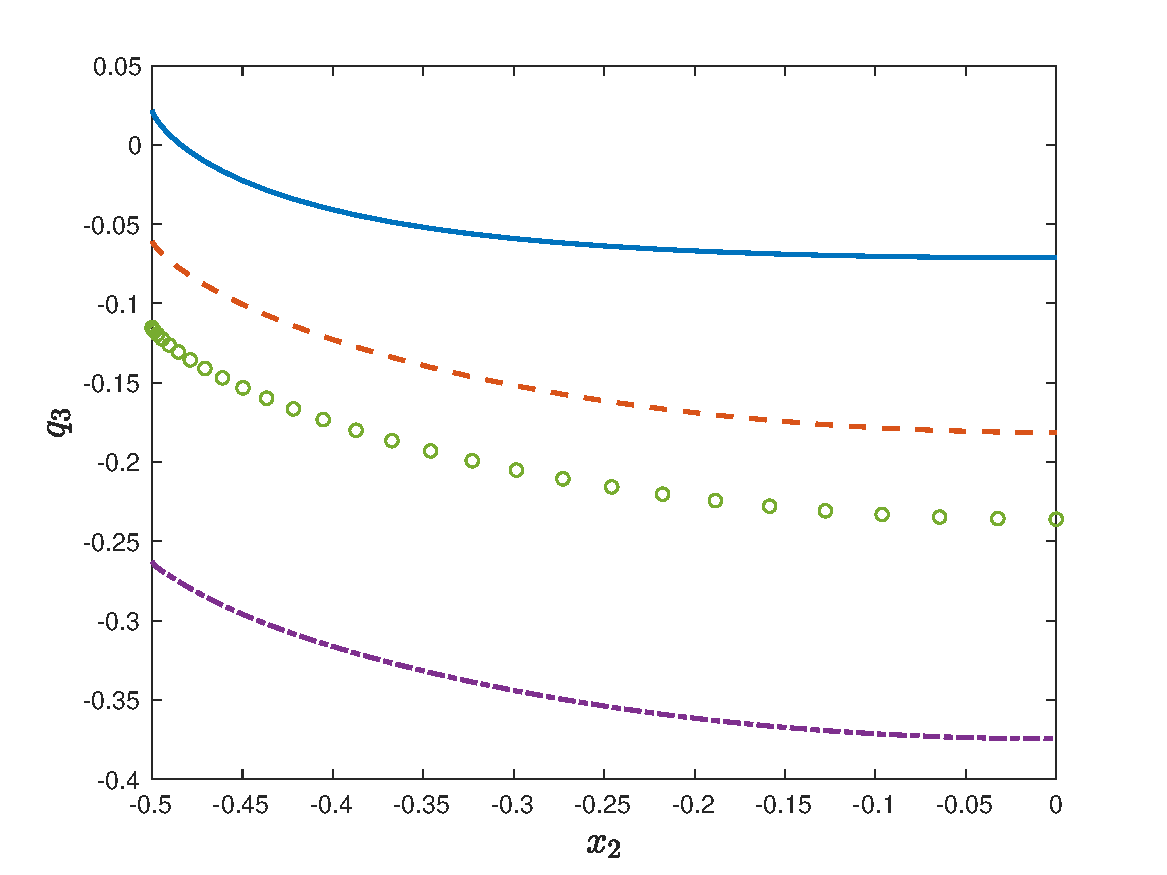
\includegraphics[scale=0.4]{LinearizedBol/IMG/Poiseuille_1D_HS2.pdf}}\\
	{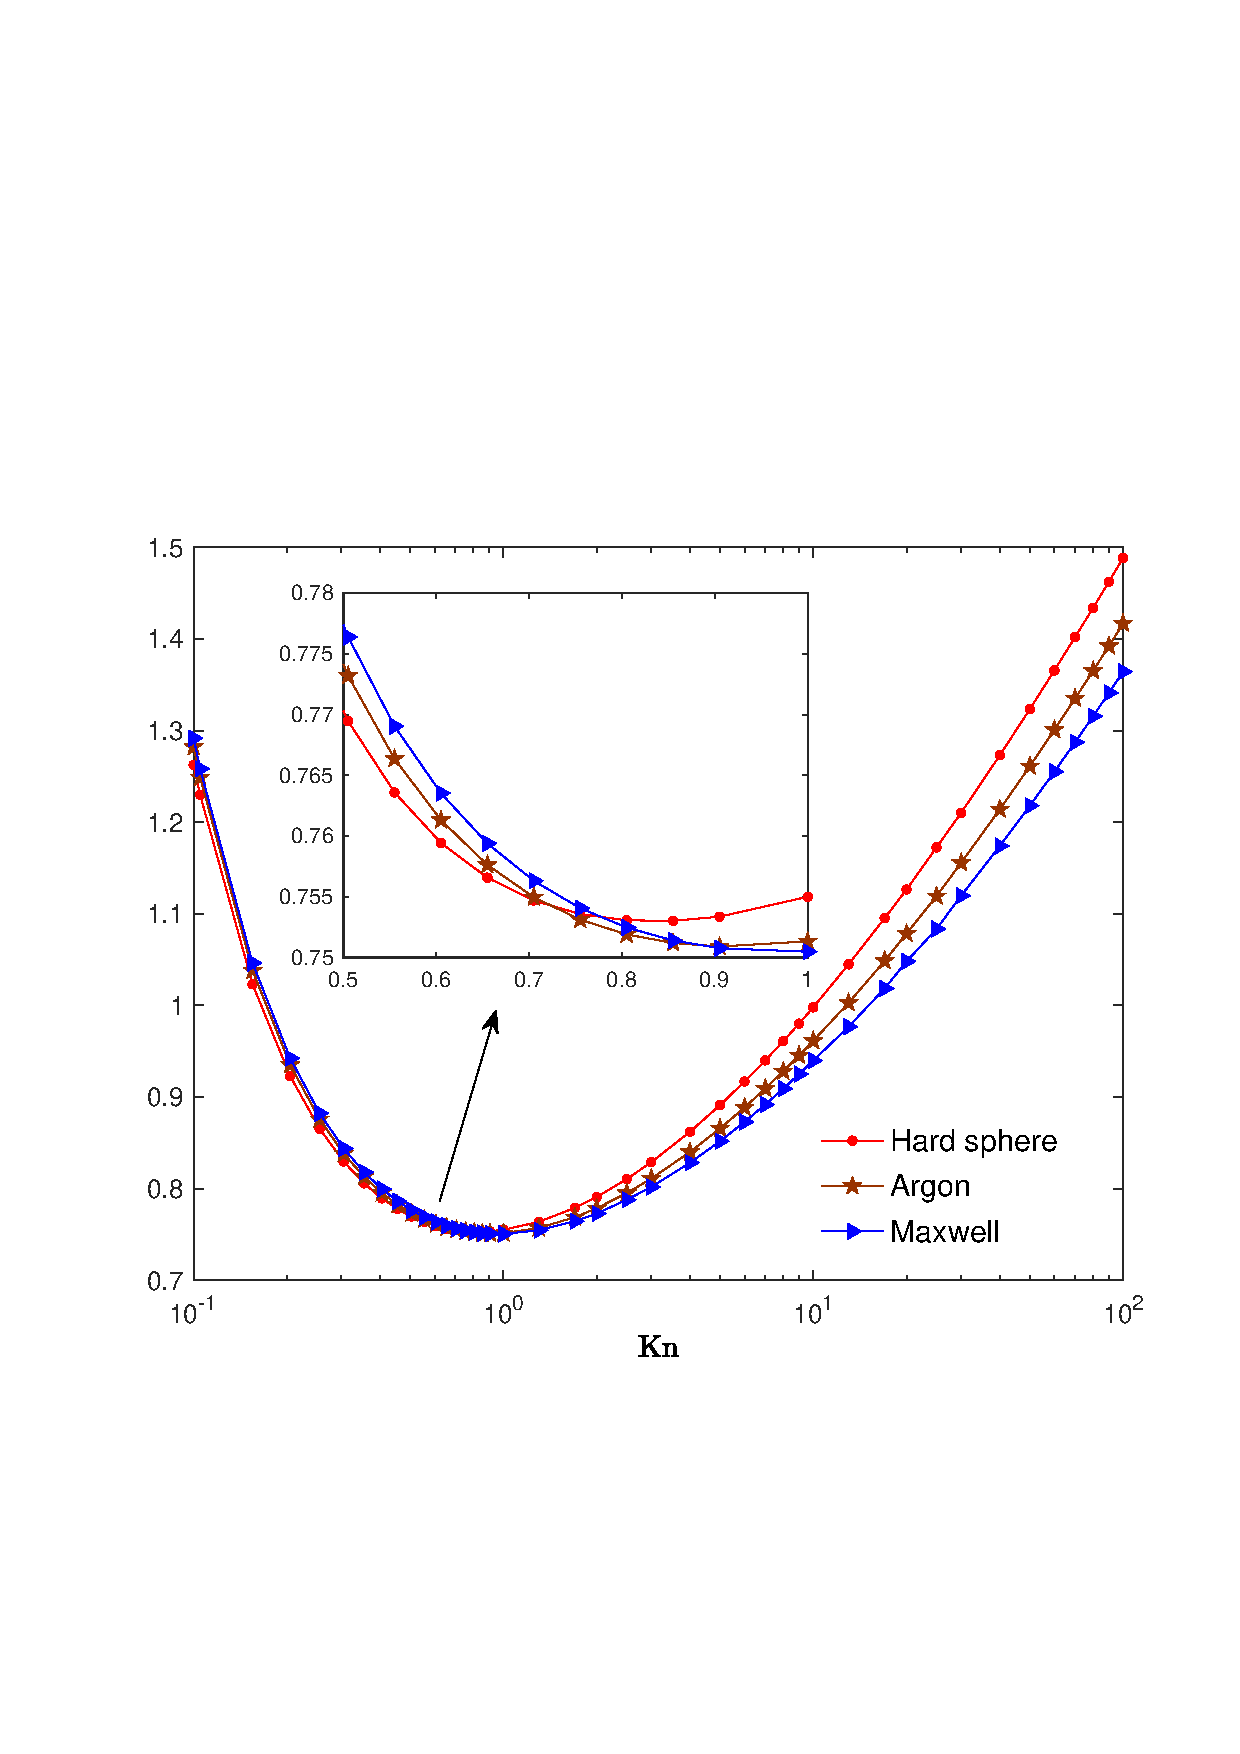
\includegraphics[scale=0.4]{LinearizedBol/IMG/pof_mass.pdf}}\quad
	{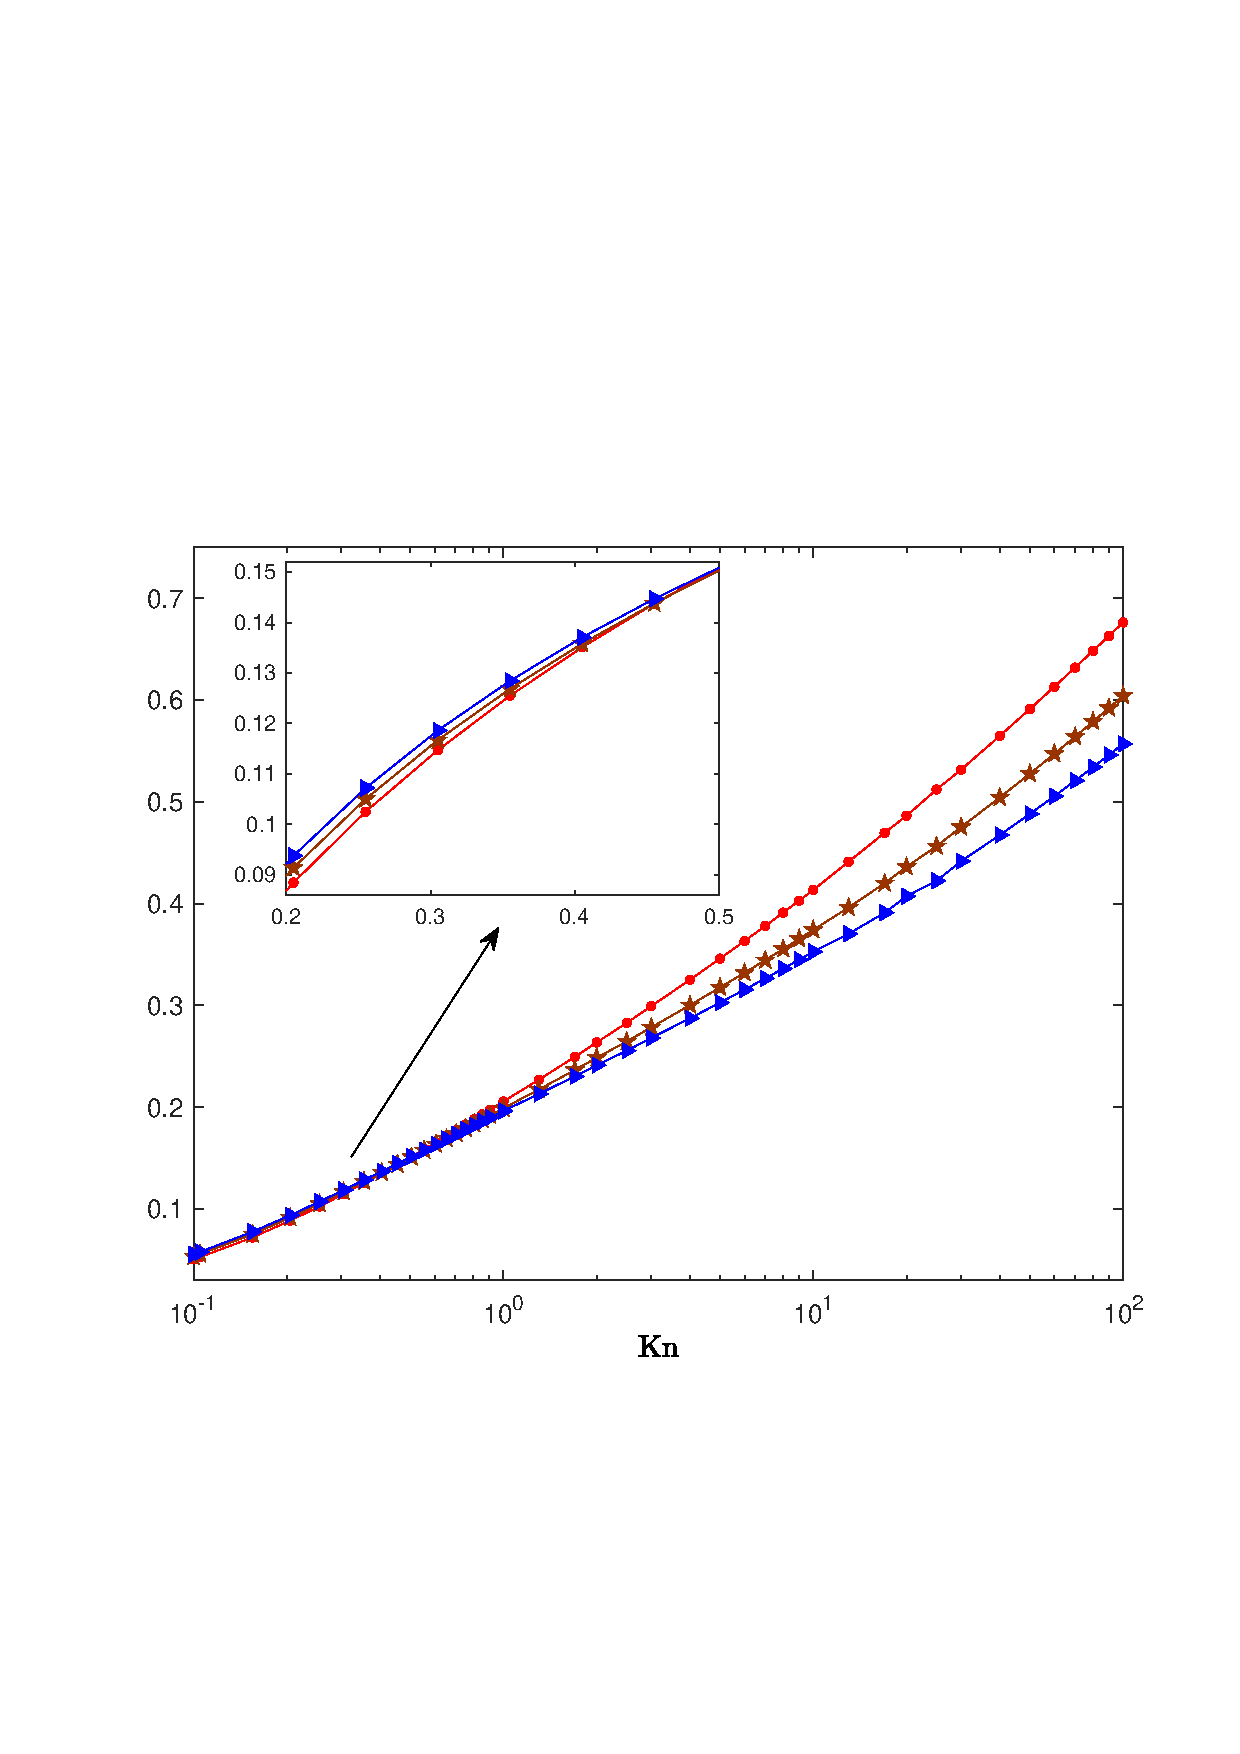
\includegraphics[scale=0.4]{LinearizedBol/IMG/pof_heat.pdf}}
	\caption{ Poiseuille gas flow between parallel plates. (Top row) Velocity and heat flux in the HS gas. (Bottom row) Comparisons in MFR (left) and HFR (right) for different inverse power-law potentials~\cite{lei_Jfm}. The viscosity index for argon is $\omega=0.81$.  } 
	\label{massheat}
\end{figure}


Because of the ``over-concentration'' in VDF~\cite{Takata2011}, numerical simulation of highly rarefied gas flows is a difficult task; for a long time the accurate numerical results have been limited to HS molecules when $\text{Kn}\lesssim20$~\cite{Ohwada_sone_1989,Doi2010}. With FSM, the LBE can be solved accurately and efficiently up to $\text{Kn}\sim10^6$. Typical VDF profiles demonstrating the over-concentration \index{velocity distribution function!over-concentration} phenomena are shown in Fig.~\ref{Onsager0}. When $\text{Kn}=1$, the marginal VDF \index{velocity distribution function!marginal} is roughly proportional to $\exp(-v_2^2)$. However, in the free-molecular \index{free-molecular flow} regime, the marginal VDF has a long tail, and its width shrinks drastically as $1/\text{Kn}$, while its amplitude scales as $\text{Kn}$. If the velocity discretization is not refined around $v_2\sim 0$, the calculated flow rates will be wrong. %which is consistent with the first-order analytical solution of Takata and Funagane~\cite{Takata2011}. 





\begin{figure}[t]
	\centering
	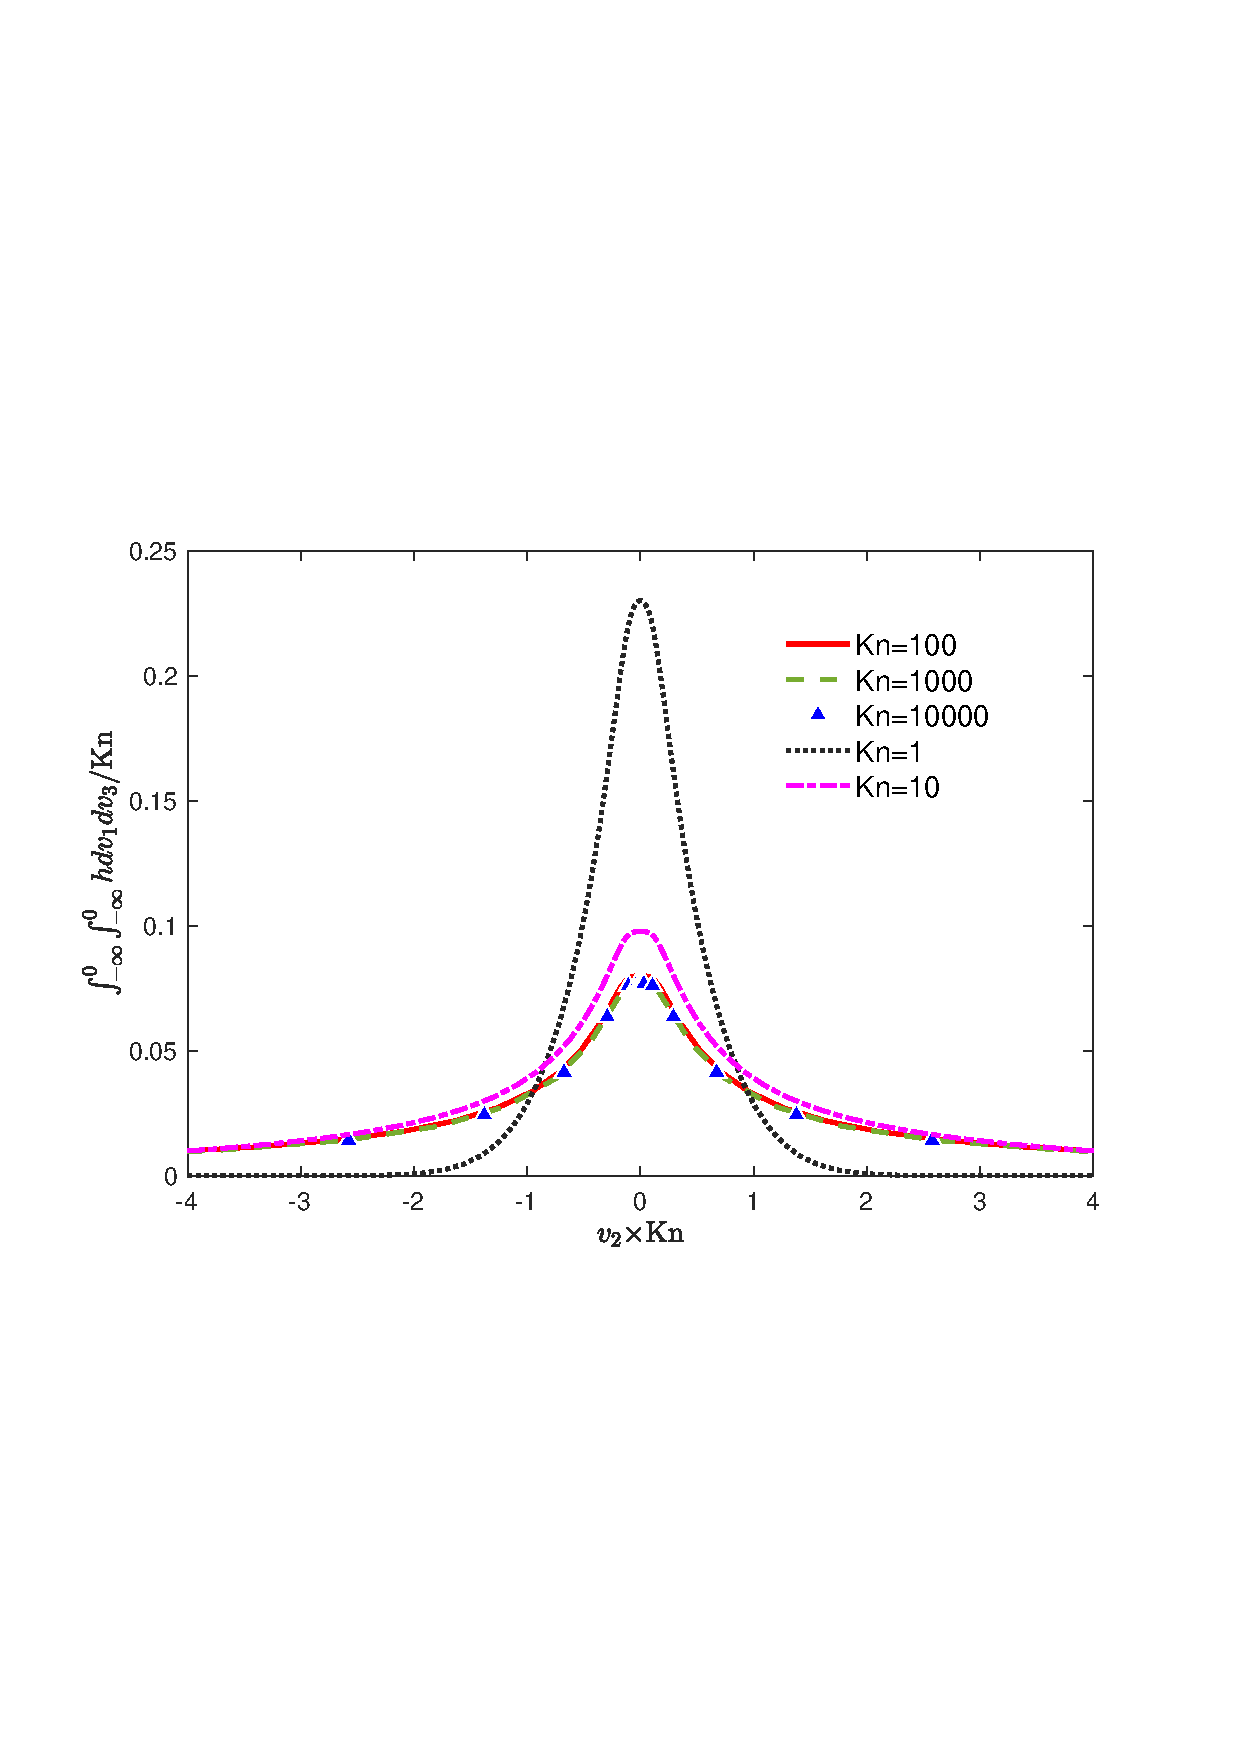
\includegraphics[width=0.6\columnwidth]{LinearizedBol/IMG/poiseuille_mm.pdf}
	\vskip 0.3cm
    \includegraphics[width=0.6\columnwidth]{LinearizedBol/IMG/thermal_VDF}
	\caption{ 
		(Top) The marginal VDF in the Poiseuille flow at the channel center. When $\text{Kn}\ge100$, the velocity distribution perpendicular to the plate shrinks as $1/\text{Kn}$, which is known as the ``over-concentration''~\cite{Takata2011}. (Bottom) 	The Onsager-Casimir relation at the mesoscopic level. Symbols: the marginal VDFs  $\iint_{-\infty}^0{} hdv_1dv_3/\text{Kn}$, where $h$ is obtained in the thermal transpiration. Lines: the marginal VDFs  $\iint_{-\infty}^0{} \left(v^2-\frac{5}{2}\right)hdv_1dv_3/\text{Kn}$, where $h$ is obtained in the Poiseuille flow.
	} 
	\label{Onsager0}
\end{figure}

%\begin{table}[t]
%	\centering
%	\caption{
%		MFR and HFR in the Poiseuille flow of HS gas between two parallel plates.
%	} \label{table_poiseuille_1d_compare} 
%	\begin{tabular}{cccccccccccc}
%		\hline
%		&  \multicolumn{2}{c}{FSM} & \multicolumn{2}{c}
%		{Ohwada \textit{et al.}~\cite{Ohwada_sone_1989}}  &
%		\multicolumn{2}{c}
%		{Takata and Funagane~\cite{Takata2011}} 
%		\\  \hline
%$8\text{Kn}/5\sqrt\pi$ & $G_P$ & $Q_p$ & $G_P$ & $Q_p$ & $G_P$ & $Q_p$\\  
%0.1    & 1.1961 & 0.0552   & 1.1930   & 0.0553  & -      &-  \\  
%0.15   & 0.9951 & 0.0761   & 0.9938   & 0.0761  & -      &-  \\  
%0.2    & 0.9007 & 0.0934   & 0.8999   & 0.0935  & -      &-  \\  
%0.3    & 0.8156 & 0.1208   & 0.8152   & 0.1209  & -      &-  \\  
%0.4    & 0.7804 & 0.1418   & 0.7801   & 0.1419  & -      &-  \\    
%0.6    & 0.7564 & 0.1729   & 0.7562   & 0.1730  & -      &-  \\
%0.8    & 0.7535 & 0.1958   & 0.7533   & 0.1958  & -      &-  \\
%1      & 0.7575 & 0.2140   & 0.7574   & 0.2140  & -      &-  \\
%1.5    & 0.7771 & 0.2477   & 0.7771   & 0.2477  & -      &-\\
%2      & 0.7991 & 0.2724   & 0.7991   & 0.2724  & -      &-\\  
%3      & 0.8399 & 0.3083   & 0.8398   & 0.3082  & -      &-\\
%4      & 0.8750 & 0.3346   & 0.8749   & 0.3345  & -      &-\\
%6      & 0.9322 & 0.3731   & 0.9321   & 0.3730  & -      &-\\
%8      & 0.9779 & 0.4016   & 0.9778   & 0.4015  & -      &-\\
%10     & 1.0160 & 0.4242   & 1.0159   & 0.4242  & 1.0159 & 0.4241  \\
%15 	 & 1.0908 & 0.4669   & 1.0908   & 0.4669  &- 	   &-        \\
%20     & 1.1478 & 0.4984   & 1.1479   & 0.4984  & 1.1477 & 0.4982  \\
%$10^2$ & 1.5143 & 0.6901   & -        &-		  & 1.5143 & 0.6900  \\
%$10^3$ & 2.1210 & 0.9960   & - 		&-		  & 2.1210 & 0.9960  \\
%$10^4$ & 2.7614 & 1.3165   & - 		&-        & 2.7615 & 1.3166  \\  
%$10^5$ & 3.4094 & 1.6405   & - 		&-        & 3.4094 & 1.6406  \\
%$10^6$ & 4.0587 & 1.9652   & - 		&-        & 4.0587 & 1.9652  \\
%		\hline
%	\end{tabular}
%\end{table}



\subsubsection{Poiseuille flow through a long duct}

Consider the Poiseuille flow in a long duct with the aspect ratio $A=S/L^2$, under the diffuse BC. Unlike the Poiseuille flow between parallel plates where the flow rates increase logarithmically at large $\text{Kn}$, here they saturate at $G_P=\mathcal{M}$ and $Q_P=\mathcal{M}/2$ when $\text{Kn}\rightarrow\infty$~\cite{loyalka1976}, where 
\begin{equation}\label{Mass_flow_rate_fm}
\begin{aligned}[b]
\mathcal{M}=\frac{1}{4\sqrt{\pi}}&\left[\frac{2(A^3+1)}{3A}-\frac{2(A^2+1)^{3/2}}{3A} \right. \\
&\left.
 +\ln\frac{(A^2+1)^{1/2}+A}{(A^2+1)^{1/2}-A}+A\ln\frac{(A^2+1)^{1/2}+1}{(A^2+1)^{1/2}-1} \right].
\end{aligned}
\end{equation}

\begin{table}[t]
	\centering
	\caption{
		MFR and HFR in the Poiseuille flow of HS gas through a rectangular channel~\cite{Wu2013PhDthesis}. Note that $\text{Kn}=5\pi{}k'/16.$ 
	} \label{table_poiseuille_2d_compare} 
		\centering
		\begin{tabular}{cccccccccccc}
			\hline
			&  \multicolumn{4}{c}{$A=1$} & \multicolumn{4}{c}
			{$A=2$}        \\  
			&  \multicolumn{2}{c}{FSM} & \multicolumn{2}{c}{Doi~\cite{Doi2010}}  
			&  \multicolumn{2}{c}{FSM} & \multicolumn{2}{c}{Doi~\cite{Doi2010}}  
			\\  \hline 
			$k'$ & $G_P$ & $Q_P$ & $G_P$ & $Q_P$ & $G_P$ & $Q_P$ & $G_P$ & $Q_P$ \\  
			0.1    & 0.6116 & 0.0445   & 0.613   & 0.045  & 0.9009  & 0.0476    & 0.905   & 0.048\\  
			%0.2    & 0.4691 & 0.0716   & 0.470   & 0.072  & 0.6676  & 0.0790    & 0.668   & 0.079\\  
			0.3    & 0.4260 & 0.0889   & 0.426   & 0.089  & 0.5950  & 0.1013    & 0.595   & 0.101 \\ 
			%0.4    & 0.4066 & 0.1010   & 0.407   & 0.101  & 0.5616  & 0.1175    & 0.562   & 0.118\\  
			0.5    & 0.3960 & 0.1103   & 0.396   & 0.110  & 0.5433  & 0.1301    & 0.544   & 0.130 \\
			%0.6    & 0.3898 & 0.1174   & 0.390   & 0.117  & 0.5322  & 0.1401    & 0.532   & 0.140 \\
			0.8    & 0.3833 & 0.1280   & 0.383   & 0.128  & 0.5203  & 0.1554    & 0.520   & 0.156 \\
			1      & 0.3811 & 0.1356   & 0.381   & 0.136  & 0.5141  & 0.1664    & 0.515   & 0.167 \\
		%	2      & 0.3806 & 0.1558   & 0.380   & 0.156  & 0.5108  & 0.1977    & 0.512   & 0.198\\  
			3      & 0.3835 & 0.1656   & 0.383   & 0.166  & 0.5148  & 0.2131    & 0.516   & 0.214 \\
			%4      & 0.3862 & 0.1717   & 0.386   & 0.172  & 0.5191  & 0.2230    & 0.520   & 0.223 \\
			5      & 0.3886 & 0.1760   & 0.388   & 0.176  & 0.5228  & 0.2300    & 0.523   & 0.230 \\
		%	6      & 0.3906 & 0.1792   & 0.390   & 0.179  & 0.5261  & 0.2352    & 0.527   & 0.236 \\
			8      & 0.3938 & 0.1837   & 0.394   & 0.184  & 0.5314  & 0.2428    & 0.532   & 0.243  \\
			10     & 0.3963 & 0.1869   & 0.396   & 0.187  & 0.5354  & 0.2481    & 0.536   & 0.248  \\
			20     & 0.4033 & 0.1948   & -       &-       & 0.5479  & 0.2613    & -       & -  \\
			50     & 0.4102 & 0.2016   & -       &-       & 0.5596  & 0.2734    & -       & -  \\
			$10^2$ & 0.4136 & 0.2048   & -       &-       & 0.5657  & 0.2791    & -       & -  \\
			$10^3$ & 0.4183 & 0.2089   & -       &-       & 0.5742  & 0.2865    & -       & - \\   
			$10^4$ & 0.4191 & 0.2095   & -       &-       & 0.5758  & 0.2878    & -       & - \\   
			$\infty$\footnote{Data in columns 4, 5, 8, and 9 are obtained from Eq.~\eqref{Mass_flow_rate_fm}.} & 0.4194 & 0.2097   & 0.4194  & 0.2097 & 0.5762  & 0.2881    & 0.5762  & 0.2881  \\
			\hline
		\end{tabular}\par
		\vspace{-0.75\skip\footins}
		\renewcommand{\footnoterule}{}
\end{table}


%This problem was first solved by the and then by the low-noise DSMC 

Nice agreement in the mass and heat flow rates of HS gas between the FSM and numerical kernel method \index{numerical kernel method}  are observed in Table~\ref{table_poiseuille_2d_compare}. To show the numerical efficiency we consider the HS gas inside a square channels; with a $25\times25$ spatial cells, $32\times32\times24$ frequency components, and $M=6$, the flow rates at $\text{Kn}_{vhs}=1$ and 10 are obtained in about 1 minute, when our Fortran code runs on a single core of an Intel Q9650 (3.0 GHz Core 2 Quad processor), while the low-noise DSMC \index{DSMC!low-noise} takes respectively 66 and 12 minutes~\cite{Doi2010,Radtke2011}. 


%.\footnote{With the general synthetic iterative scheme in Chapter~\ref{chap:GSIS}, we can achieve the efficiency for any value of Knudsen number, while the simulation time for conventional iterative scheme and low-variance DSMC increases dramatically when $Kn$ decreases.}. 






\subsection{Onsager-Casimir relation} \index{Onsager-Casimir relation}


%\begin{figure}[t]
%	\centering
%	\includegraphics[scale=0.5]{thermal_VDF}
%	\caption{ 
%		The Onsager-Casimir relation at the mesoscopic level. Symbols: the marginal VDFs  $\iint_{-\infty}^0{} hdv_1dv_3/\text{Kn}$, where $h$ is obtained in the thermal transpiration. Lines: the marginal VDFs  $\iint_{-\infty}^0{} \left(v^2-\frac{5}{2}\right)hdv_1dv_3/\text{Kn}$, where $h$ is obtained in the Poiseuille flow.
%	} 
%	\label{Onsager}
%\end{figure}


The Onsager-Casimir relation states that the MFR in the thermal transpiration is equal to the HFR in the Poiseuille flow. In the numerical simulation we find that this relation is held with the absolute error smaller than $10^{-4}$. 

Takata and Funagane~\cite{Takata2011} made the important observation that at large $\text{Kn}$, $u_3[h_T]$ and $q_3[h_P]$ are even identical at the level of spatial profile:
\begin{equation}
u_3[h_T]=q_3[h_P]+O\left(\frac{(\ln{\text{Kn}})^2}{\text{Kn}}\right).
\end{equation}
Our numerical results in Fig.~\ref{Onsager0} further show that the agreement is even at the mesoscopic level:
\begin{equation}
h_T\approx\left({v}^2-\frac{5}{2}\right)h_P.
\end{equation} 

%
%The asymptotic mass flow rates at large $\text{Kn}$ in the Poiseuille flow and thermal transpiration have also been obtained~\cite{Takata2011}. It has been found that they increase logarithmically with respect to $\text{Kn}$. For the heat flow rate in the thermal transpiration, we find it can also be well fitted by the logarithmic function of $\text{Kn}$:
%\begin{equation}
%Q_T=0.6345\ln(\text{Kn})+Q_0
%\end{equation} 
%in the region $10^5<\text{Kn}<2\times10^6$, where the constant $Q_0$ is 0.2679, 0.1762, 0.07371, and -0.09903 for the HS molecules, helium, argon, and the Maxwell molecules, respectively.



\section{Influence of intermolecular potential}

Note that except for the HS gas, the collision kernels in the previous chapter are modeled to recover the shear viscosity, rather than calculated directly from the intermolecular potential. Here we extend the FSM to solve the LBE with the collision kernel directly calculated from the Lennard-Jones potential~\eqref{Lennard_Jones_chapter}, rather than using the modeled kernel~\eqref{kernel_spectral}. 





%When $\rho_r$ is determined, the integral given by Eq.~\eqref{psi_expression} is calculated numerically, where $s\in[0,\text{max}(\sqrt{3}\xi)]$ is uniformly discretized into 8000 sections. 




%\begin{figure}[thbp]
%	\centering
%	\includegraphics[scale=0.5]{CouetteFull_LJ}
%	\caption{Profiles of the density, velocity, temperature, and heat flux in the nonlinear Couette flow at $\delta_{rp}=0.1$. Dash-dotted lines: HS gas; Solid lines: He; Dashed lines: Xe. }
%	\label{CouetteFull}
%\end{figure}




\begin{table}
	\caption{Mass flow rate $G_P$ and heat flow rate $Q_P$ in the Poiseuille flow between parallel infinite plates, when the Lennard-Jones potential is considered~\cite{wuPoF2015}.   }
	\centering
	\begin{tabular}{ccccccccccccccccccccc}
		\hline 
		& \multicolumn{2}{c}{He}
		& \multicolumn{2}{c}{Ne}  
		& \multicolumn{2}{c}{Ar} 
		& \multicolumn{2}{c}{Kr}  
		& \multicolumn{2}{c}{Xe} \\ 
		\hline 
$\delta_{rp}$ & $G_P$  &$Q_P$ & $G_P$ &$Q_P$  & $G_P$  &$Q_P$  &$G_P$ &$Q_P$  & $G_P$  & $Q_P$   \\ \hline 
		$0.01$ & 2.713& 1.152& 2.607& 1.070& 2.535& 1.057& 2.538& 1.065& 2.547& 1.072  \\
		$0.02$ & 2.432& 1.021& 2.362& 0.961& 2.292& 0.930& 2.286& 0.933& 2.290& 0.938  \\
		$0.025$ &2.348& 0.981& 2.289& 0.929& 2.219& 0.893& 2.211& 0.894& 2.214& 0.898  \\
		$0.04$ & 2.180& 0.900& 2.141& 0.862& 2.076& 0.819& 2.063& 0.815& 2.064& 0.818  \\
		$0.05$ & 2.105& 0.863& 2.074& 0.831& 2.011& 0.785& 1.998& 0.780& 1.998& 0.782  \\
		$0.10$ & 1.892& 0.749& 1.879& 0.732& 1.829& 0.688& 1.815& 0.679& 1.813& 0.679  \\
		$0.20$ & 1.713& 0.637& 1.708& 0.629& 1.677& 0.596& 1.666& 0.586& 1.663& 0.584  \\
		$0.25$ &1.665 & 0.601& 1.661& 0.595& 1.636& 0.566& 1.626& 0.557& 1.624& 0.555  \\
		$0.40$ & 1.581& 0.526& 1.579& 0.523& 1.564& 0.504& 1.558& 0.497& 1.556& 0.495  \\
		$0.50$ & 1.550& 0.491& 1.549& 0.489& 1.539& 0.474& 1.534& 0.468& 1.532& 0.466  \\
		$1.00$ & 1.505& 0.385& 1.505& 0.384& 1.505& 0.380& 1.505& 0.378& 1.505& 0.377  \\
		$1.60$ & 1.532& 0.315& 1.533& 0.315& 1.537& 0.315& 1.540& 0.316& 1.541& 0.315  \\
		$2.00$ & 1.568& 0.282& 1.568& 0.283& 1.575& 0.285& 1.579& 0.286& 1.580& 0.286  \\
		$2.50$ & 1.622& 0.251& 1.623& 0.251& 1.630& 0.254& 1.636& 0.256& 1.637& 0.257  \\
		$4.00$ & 1.817& 0.188& 1.818& 0.189& 1.828& 0.193& 1.835& 0.196& 1.838& 0.197  \\
		$5.00$ & 1.960& 0.161& 1.961& 0.162& 1.972& 0.166& 1.980& 0.169& 1.983& 0.170  \\
		$10.0$ & 2.732& 0.093& 2.732& 0.093& 2.743& 0.097& 2.752& 0.099& 2.756& 0.100  \\
		\hline
	\end{tabular} 
	\label{table_poiseuille_lj_mass} 
\end{table}



The numerical results in Table~\ref{table_poiseuille_lj_mass} shows that different parameters in the Lennard-Jones potential~\eqref{Lennard_Jones_chapter} lead to different flow rate, especially when the rarefaction parameter is small. 
 
%For $\delta_{rp}\ge0.025$, the difference between our results and those of Sharipov and Bertoldo is $\lesssim1\%$, which increases to about 2\% at $\delta_{rp}=0.01$. These differences are small, as the numerical accuracy of the discrete velocity method is about 0.8\%~\cite{Sharipov2009}. 


%\leir{At the temperature $T_0$, it is known that the equivalent viscosity index of He, Ne, Ar, Kr, and Xe are 0.66, 0.66, 0.81, 0.8, and 0.85, respectively.}






\section{Cercignani-Lampis boundary condition}
\index{boundary condition!Cercignani-Lampis}

% data used in Chapter 2: kinetic boundary conditions

We present the LBE solutions for the Poiseuille flow between two plates and through a circular cross section~\cite{WuStruchtrupJFM2017}. Although this classical problem has been investigated extensively, accurate numerical results based on the LBE and the Cercignani-Lampis  BC is scarce. 

%With the state-of-the-art numerical method, the mass and heat flow rates of the Poiseuille flow and thermal transpiration are obtained with the Cercignani-Lampis BC, which provides critical data to assess the gas kinetic boundary conditions in Chapter~\ref{chap:BoundaryCondition}.

%
%For the Cercignani-Lampis  BC, the scattering kernel~\eqref{CL} is simplified
%to~\citep{Sharipov2002CL,Sharipov2003CL,SharipovCL3}: 
%\begin{equation}
%R_{CL}(\bm{v}^{\prime}\rightarrow \bm{v})=R_n(v_n^{\prime}\rightarrow%
%{v_n})R_t(\bm{v}_t^{\prime}\rightarrow{\bm{v}_t}),
%\end{equation}
%where 
%\begin{equation}  
%\begin{aligned}[b] R_n(v_n'\rightarrow{v_n})=&\frac{2v_n}{\alpha_n}
%I_0\left(2\frac{\sqrt{1-\alpha_n}v_nv_n'}{\alpha_n}\right)\exp\left\{-%
%\frac{[v_n^2+(1-\alpha_n)v_n']^2}{\alpha_n} \right\},\\
%R_t(\bm{v}_t'\rightarrow{\bm{v}_t})=&\frac{1}{\pi\alpha_t(2-%
%	\alpha_t)}\exp\left[-\frac{|\bm{v}_t-(1-\alpha_t)\bm{v}_t'|^2}{%
%	\alpha_t(2-\alpha_t)} \right]. 
%\end{aligned}
%\end{equation}


\subsection{Poiseuille flow through parallel plates} 

Table~\ref{table_poiseuille_1d_BC} shows the flow rates for HS molecules. When the rarefaction parameter $\delta_{rp}$ and the EAC \index{accommodation coefficient!energy} $\alpha _{n}$ are fixed, the MFR increases rapidly when the TMAC $\alpha _{t}$ decreases. However, the influence of $\alpha _{n}$ on MFR is limited. 
%When $\alpha _{t}$ and $\delta_{rp}$ are fixed, the MFR decreases slightly when $\alpha _{n}$ increases. For instance, when $\delta_{rp} =0.01$, the MFR is decreased by 10\% when $\alpha _{n}$ is increased from 0.25 to 1; as $\delta_{rp} $ increases, this influence becomes weaker and weaker. 


	

\begin{table}
	\centering
	\caption{Dimensionless flow rates in the Poiseuille flow of HS molecules between two parallel plates~\cite{WuStruchtrupJFM2017}. The Cercignani-Lampis BC is used, but the data in the last two columns are from the Maxwell BC. }
\begin{tabular}{clccclccccccc}
	\hline
	&  & ${G}_P$ & ${Q}_P$ & ${G}_P$ & ${Q}_P$ & ${G}_P$ & ${Q}_P$ & ${G}_P$
	& ${Q}_P$ & ${G}_P$ & ${Q}_P$   \\ 
	$\delta_{rp}$ & $\alpha_t$ & \multicolumn{2}{c}{$\alpha_n$=0.25} & 
	\multicolumn{2}{c}{$\alpha_n$=0.5} & \multicolumn{2}{c}{$\alpha_n$=0.75} & 
	\multicolumn{2}{c}{$\alpha_n$=1} & \multicolumn{2}{c}{$\alpha_M=\alpha_t$} 
	\\ 
	\hline
	0.01 & 0.5 & 5.115 & 1.699 & 4.871 & 1.499 & 4.752 & 1.390 & 4.684 & 1.322 & 
	6.844 & 2.991   \\ 
	& 1 & 2.911 & 1.320 & 2.911 & 1.320 & 2.911 & 1.320 & 2.911 & 1.320 & 2.911
	& 1.320   \\ 
	& 1.5 & 2.084 & 1.122 & 2.196 & 1.205 & 2.265 & 1.265 & 2.320 & 1.319 &  & 
	  \\ 
	0.1 & 0.5 & 3.996 & 1.098 & 3.854 & 0.953 & 3.774 & 0.866 & 3.724 & 0.807 & 
	4.389 & 1.570   \\ 
	& 1 & 1.951 & 0.801 & 1.951 & 0.801 & 1.951 & 0.801 & 1.951 & 0.801 & 1.951
	& 0.801   \\ 
	& 1.5 & 1.200 & 0.634 & 1.270 & 0.699 & 1.319 & 0.749 & 1.360 & 0.796 &  &   \\ 
	0.2 & 0.5 & 3.710 & 0.906 & 3.616 & 0.798 & 3.558 & 0.726 & 3.519 & 0.675 & 
	3.907 & 1.211   \\ 
	& 1 & 1.747 & 0.667 & 1.747 & 0.667 & 1.747 & 0.667 & 1.747 & 0.667 & 1.747
	& 0.667   \\ 
	& 1.5 & 1.037 & 0.525 & 1.086 & 0.577 & 1.123 & 0.620 & 1.156 & 0.661 &  &   \\ 
	1 & 0.5 & 3.308 & 0.458 & 3.297 & 0.435 & 3.288 & 0.415 & 3.280 & 0.398 & 
	3.327 & 0.529   \\ 
	& 1 & 1.507 & 0.389 & 1.507 & 0.389 & 1.507 & 0.389 & 1.507 & 0.389 & 1.507
	& 0.389   \\ 
	& 1.5 & 0.894 & 0.336 & 0.901 & 0.351 & 0.908 & 0.366 & 0.915 & 0.381 &  &   \\ 
	2 & 0.5 & 3.340 & 0.300 & 3.339 & 0.296 & 3.338 & 0.292 & 3.337 & 0.288 & 
	3.347 & 0.328   \\ 
	& 1 & 1.564 & 0.281 & 1.564 & 0.281 & 1.564 & 0.281 & 1.564 & 0.281 & 1.564
	& 0.281   \\ 
	& 1.5 & 0.970 & 0.265 & 0.971 & 0.268 & 0.971 & 0.272 & 0.972 & 0.275 &  &  \\ 
%	3.5 & 0.5 & 3.518 & 0.201 & 3.517 & 0.203 & 3.516 & 0.204 & 3.515 & 0.206 & 
%	3.524 & 0.212   \\ 
%	& 1 & 1.742 & 0.202 & 1.742 & 0.202 & 1.742 & 0.202 & 1.742 & 0.202 & 1.742
%	& 0.202  \\ 
%	& 1.5 & 1.148 & 0.203 & 1.149 & 0.202 & 1.150 & 0.200 & 1.150 & 0.198 &  &  \\ 
	10 & 0.5 & 4.522 & .0834 & 4.514 & .0861 & 4.508 & .0887 & 4.503 & .0912 & 
	4.535 & .0843  \\ 
	& 1 & 2.729 & .0900 & 2.729 & .0900 & 2.729 & .0900 & 2.729 & .0900 & 2.729
	& .0900   \\ 
	& 1.5 & 2.120 & .0962 & 2.127 & .0938 & 2.133 & .0913 & 2.138 & .0889 &  &   \\ 
	20 & 0.5 & 6.162 & .0437 & 6.151 & .0454 & 6.142 & .0470 & 6.133 & .0485 & 
	6.177 & .0437   \\ 
	& 1 & 4.360 & .0480 & 4.360 & .0480 & 4.360 & .0480 & 4.360 & .0480 & 4.360
	& .0480  \\ 
	& 1.5 & 3.743 & .0519 & 3.752 & .0505 & 3.761 & .0490 & 3.769 & .0474 &  &   \\ 
	100 & 0.5 & 19.47 & .0091 & 19.45 & .0094 & 19.44 & .0098 & 19.43 & .0102 & 
	19.49 & .0090   \\ 
	& 1 & 17.66 & .0101 & 17.66 & .0101 & 17.66 & .0101 & 17.66 & .0101 & 17.66
	& .0101   \\ 
	& 1.5 & 17.03 & .0110 & 17.05 & .0107 & 17.06 & .0103 & 17.07 & .0100 &  & \\
	\hline
\end{tabular}%
	\label{table_poiseuille_1d_BC}
\end{table}




The variation of HFR with respect to $\alpha _{n}$ and $\alpha _{t}$ is complicated. First, when $\alpha _{n}$ and $\delta_{rp}$ are fixed, the HFR increases slightly with $\alpha _{t}$ when $\delta_{rp} $ is large, while it increases with decreasing $\alpha _{t}$ when  $\delta_{rp}$ is small. Second, when $\alpha _{t}=1$ and $\delta_{rp} $ is fixed, the HFR does not change with $\alpha _{n}$: in fact, in this case the Cercignani-Lampis  BC is reduced to the diffuse  BC~\citep{Sharipov2002CL}. Third, when $\alpha_{t}(\neq1)$ and $\delta_{rp} $ are fixed, the HFR increases slightly with $\alpha _{n}$ when $\delta_{rp}$ is large, but it increases with decreasing $\alpha _{n}$ when $\delta_{rp}$ small. 

The influence of intermolecular potential is visualized in Fig.~\ref{Chapter_BC_Pois1D}, where we choose xenon and helium, as the results of other noble gases are similar. Large difference is found at small rarefaction parameter. For example, when $\delta_{rp} =0.01$, the relative differences in the MFR and HFR between HS gas and xenon are about 12\% and 23\%, respectively, when the Cercignani-Lampis  BC with $\alpha _{n}=1$ and $\alpha _{t}=0.75$ is used. 




\begin{figure}[t]
	\centering
	{	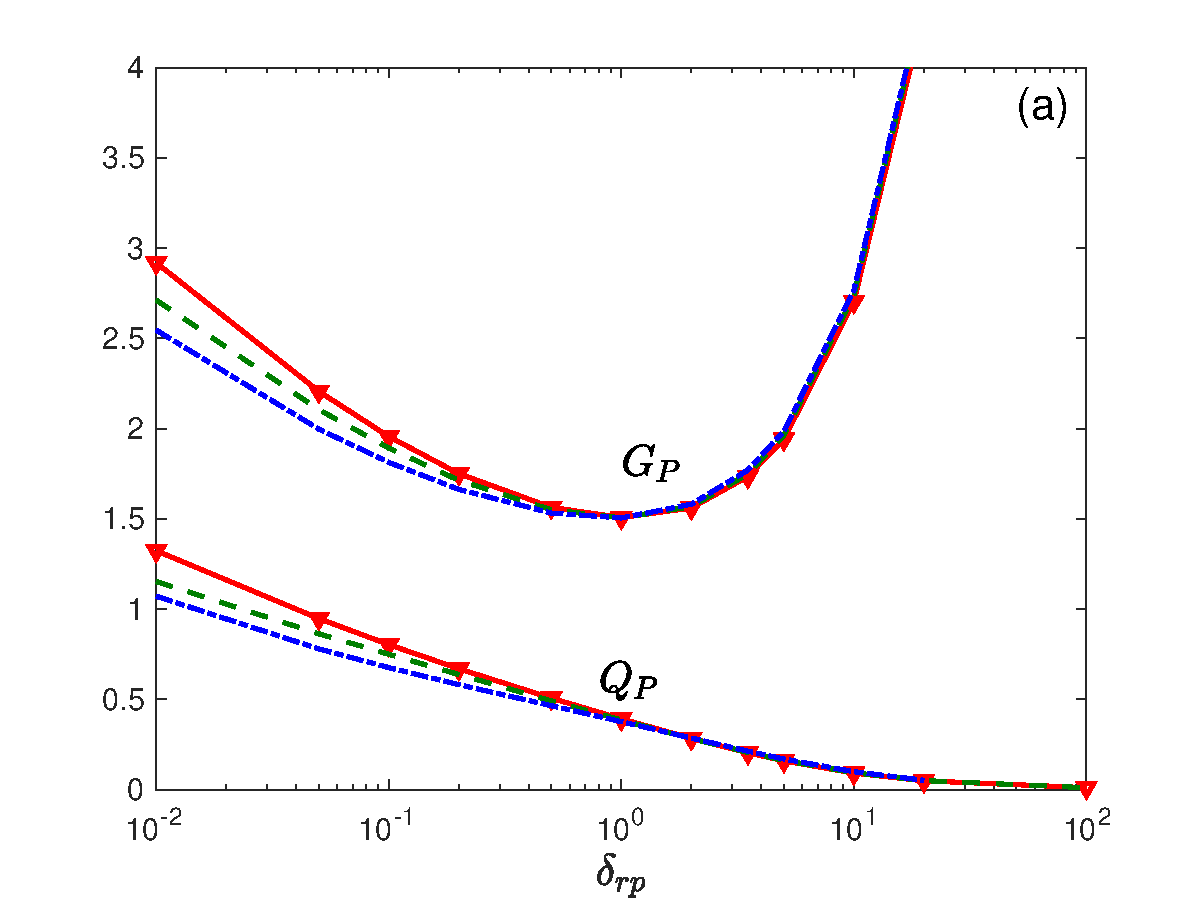
\includegraphics[width=0.48\columnwidth]{LinearizedBol/IMG/BC_Fig2a}}
	{	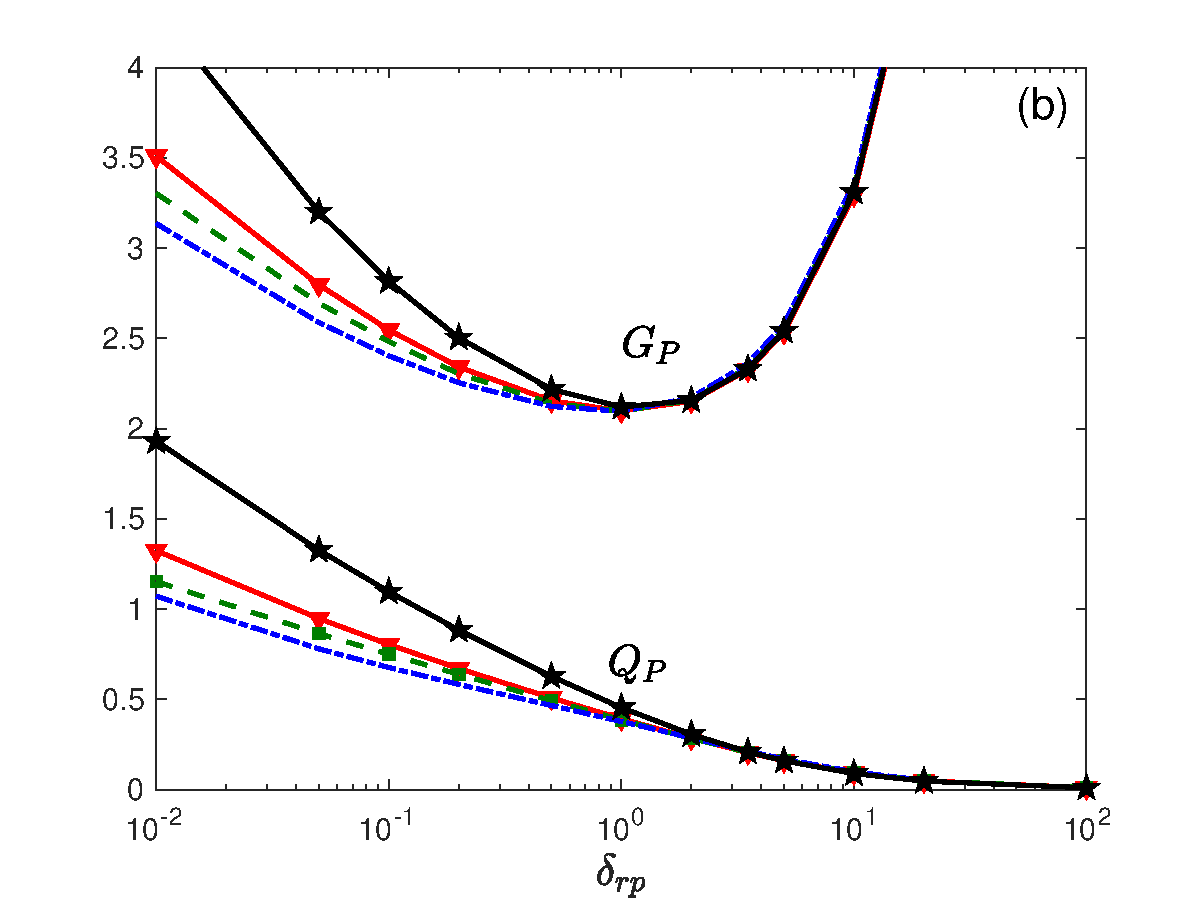
\includegraphics[width=0.48\columnwidth]{LinearizedBol/IMG/BC_Fig2b}}\\
	\vskip 0.3cm
	{	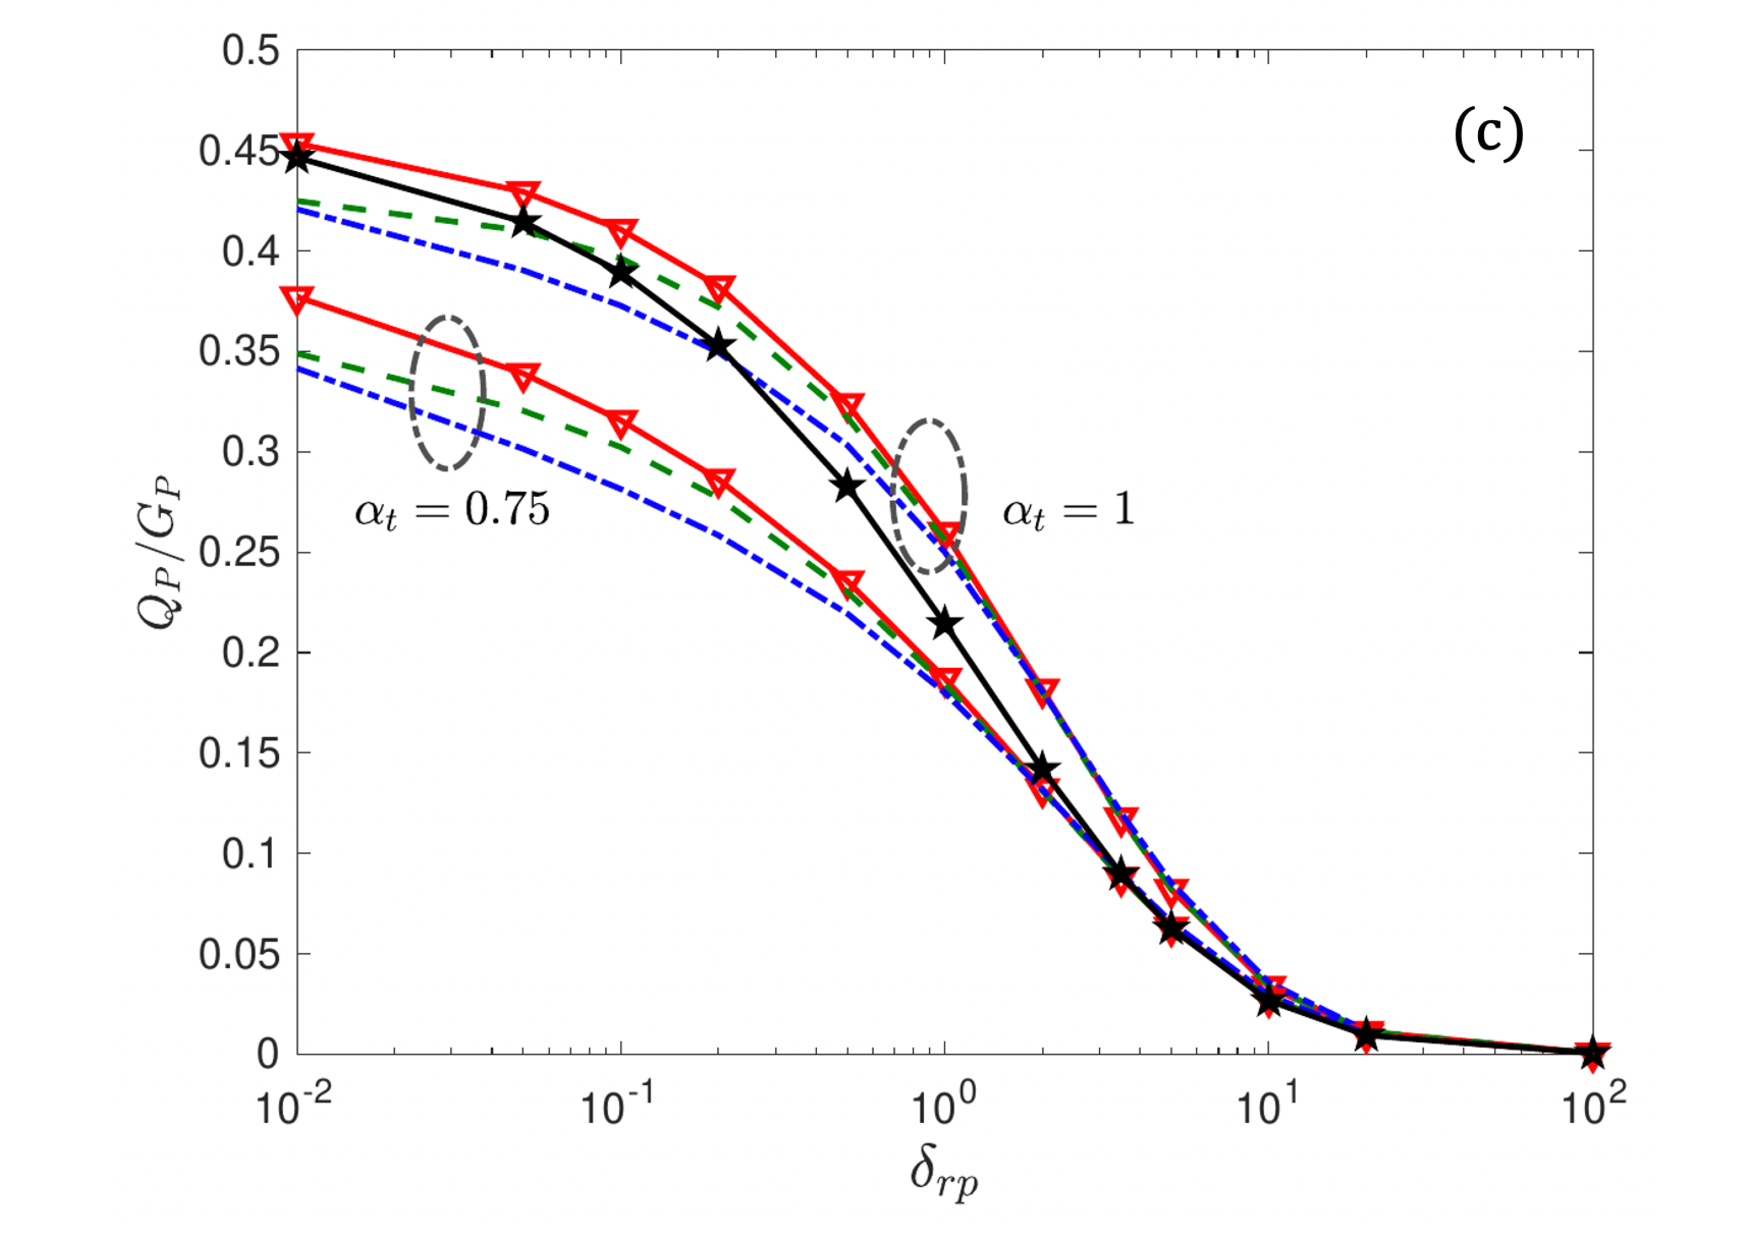
\includegraphics[width=0.6\columnwidth]{LinearizedBol/IMG/BC_Fig2c}}
	\caption{
		Flow rates in the Poiseuille flow between two parallel plates~\cite{WuStruchtrupJFM2017}. Triangles: HS gas. Dashed lines: He. Dash-dotted lines: Xe. When the Lennard-Jones potential is used, the wall temperature is $T_w=300$~K. In the Cercignani-Lampis BC, $\alpha_n=1$,  (a) $\alpha_t=1$ and (b) $\alpha_t=0.75$. In the Maxwell BC, $\alpha_M=0.75$ is used (Pentagrams). (c) The exponent of thermal pressure difference, i.e., the ratio of MFR $G_T/G_P$, or $Q_P/G_P$ as per the Onsager-Casimir relation. 
	} 
	\label{Chapter_BC_Pois1D}
\end{figure}

Figure~\ref{Chapter_BC_Pois1D}(c) shows the exponent of thermalmolecular pressure difference \index{thermalmolecular pressure difference} (TPD), which is an important parameter determining the performance of a Knudsen pump. 
In the range of $\delta_{rp}$ considered, the HS gas has the largest TPD, while xenon has the smallest. This difference increases when $\delta_{rp} $ decreases. In the Cercignani-Lampis  BC, when $\delta_{rp}$ is fixed, the TPD exponent decreases with $\alpha _{t}$. In the diffuse  BC, when the TMAC $\alpha _{M}$ decreases, the TPD exponent decreases at large values of $\delta_{rp}$, but at free-molecular flow regime, $\alpha _{M}$ does not have any influence on the TPD exponent.

%\leir{define the TPD equation here }

\begin{table}[pt]
	\centering
	\caption{Dimensionless flow rates in the Poiseuille flow of HS molecules through a circular tube, using the Cercignani-Lampis BC.  The characteristic length $L$ is the radius of circular cross section~\cite{WuStruchtrupJFM2017}.}
	\begin{tabular}{clccclccccccc}
		\hline
		&  & ${G}_P$ & ${Q}_P$ & ${G}_P$ & ${Q}_P$ & ${G}_P$ & ${Q}_P$ & ${G}_P$
		& ${Q}_P$  \\ 
		$\delta_{rp}$ & $\alpha_t$ & \multicolumn{2}{c}{$\alpha_n$=0.25} & 
		\multicolumn{2}{c}{$\alpha_n$=0.5} & \multicolumn{2}{c}{$\alpha_n$=0.75} & 
		\multicolumn{2}{c}{$\alpha_n$=1}   \\
		\hline 
	%	0 & 0.5 & 3.401 & 1.026 & 3.356 & 0.912 & 3.328 & 0.838 & 3.309 & 0.786   \\ 
	%	& 1 & 1.504 & 0.752 & 1.504 & 0.752 & 1.504 & 0.752 & 1.504 & 0.752 
	%	\\ 
	%	& 1.5 & 0.838 & 0.608 & 0.856 & 0.646 & 0.871 & 0.684 & 0.887 & 0.725   \\ 
		0.01 & 0.5 & 3.363 & 0.989 & 3.321 & 0.881 & 3.295 & 0.809 & 3.277 & 0.759   \\ 
		& 1 & 1.472 & 0.725 & 1.472 & 0.725 & 1.472 & 0.725 & 1.472 & 0.725 
		\\ 
		& 1.5 & 0.809 & 0.584 & 0.825 & 0.620 & 0.840 & 0.657 & 0.855 & 0.697   \\ 
		0.1 & 0.5 & 3.251 & 0.837 & 3.227 & 0.763 & 3.210 & 0.709 & 3.198 & 0.669   \\ 
		& 1 & 1.397 & 0.634 & 1.397 & 0.634 & 1.397 & 0.634 & 1.397 & 0.634 
		\\ 
		& 1.5 & 0.753 & 0.516 & 0.763 & 0.545 & 0.773 & 0.574 & 0.784 & 0.607   \\ 
		0.5 & 0.5 & 3.181 & 0.574 & 3.176 & 0.553 & 3.172 & 0.536 & 3.169 & 0.520 \\ 
		& 1 & 1.381 & 0.492 & 1.381 & 0.492 & 1.381 & 0.492 & 1.381 & 0.492 \\ 
		& 1.5 & 0.767 & 0.432 & 0.770 & 0.443 & 0.772 & 0.455 & 0.775 & 0.468 \\ 
		1 & 0.5 & 3.233 & 0.432 & 3.232 & 0.429 & 3.231 & 0.426 & 3.230 & 0.423 \\ 
		& 1 & 1.448 & 0.403 & 1.448 & 0.403 & 1.448 & 0.403 & 1.448 & 0.403 \\ 
		& 1.5 & 0.845 & 0.379 & 0.847 & 0.380 & 0.847 & 0.383 & 0.848 & 0.385 \\ 
		2 & 0.5 & 3.423 & 0.295 & 3.420 & 0.300 & 3.418 & 0.305 & 3.417 & 0.309 \\ 
		& 1 & 1.639 & 0.298 & 1.639 & 0.298 & 1.639 & 0.298 & 1.639 & 0.298 \\ 
		& 1.5 & 1.038 & 0.301 & 1.040 & 0.297 & 1.042 & 0.293 & 1.043 & 0.288  \\ 
		5 & 0.5 & 4.113 & 0.152 & 4.105 & 0.157 & 4.098 & 0.162 & 4.093 & 0.167 \\ 
		& 1 & 2.319 & 0.164 & 2.319 & 0.164 & 2.319 & 0.164 & 2.319 & 0.164 \\ 
		& 1.5 & 1.708 & 0.175 & 1.715 & 0.170 & 1.721 & 0.165 & 1.726 & 0.161  \\ 
		10 & 0.5 & 5.333 & .0835 & 5.322 & .0868 & 5.313 & .0899 & 5.305 & .0929  \\ 
		& 1 & 3.531 & .0917 & 3.531 & .0917 & 3.531 & .0917 & 3.531 & .0917 \\ 
		& 1.5 & 2.913 & .0992 & 2.923 & .0963 & 2.932 & .0934 & 2.939 & .0904 \\ 
		20 & 0.5 & 7.815 & .0437 & 7.802 & .0456 & 7.791 & .0472 & 7.782 & .0489 \\ 
		& 1 & 6.007 & .0484 & 6.007 & .0484 & 6.007 & .0484 & 6.007 & .0484	\\ 
		& 1.5 & 5.385 & .0527 & 5.396 & .0511 & 5.406 & .0495 & 5.416 & .0479  \\ 
		50 & 0.5 & 15.30 & .0179 & 15.28 & .0187 & 15.27 & .0194 & 15.26 & .0201  \\ 
		& 1 & 13.49 & .0200 & 13.49 & .0200 & 13.49 & .0200 & 13.49 & .0200 
		\\ 
		& 1.5 & 12.86 & .0218 & 12.87 & .0212 & 12.89 & .0205 & 12.89 & .0198  \\ 
		100 & 0.5 & 27.78 & .0090 & 27.77 & .0094 & 27.75 & .0098 & 27.74 & .0101   \\ 
		& 1 & 25.97 & .0101 & 25.97 & .0101 & 25.97 & .0101 & 25.97 & .0101 
		\\ 
		& 1.5 & 25.34 & .0110 & 25.35 & .0107 & 25.37 & .0103 & 25.38 & .0100  \\
		\hline
	\end{tabular}%
	\label{table_poiseuille_tube_compare}
\end{table}

%Fig.~\ref{Thermaltube} shows the influence of  intermolecular potential on the MFR in thermal transpiration. For $\delta_{rp} >0.5$, the HS model underpredicts the MFR of the Lennard-Jones potentials, say, when $\delta_{rp} =10$, by about 8\% and 4\% for argon and helium, respectively. When $\delta_{rp} <0.5$, however, the HS model overpredicts the MFR. When $\delta_{rp} \rightarrow 0$, the intermolecular potential has no influence on the dimensionless mass flow rate. On the other hand, the influence of intermolecular potential in the MFR of  Poiseuille flow is within 2\% for all the rarefaction parameters considered.


\subsection{Poiseuille flow through long tube}

For flows through circular cross sections, the polar coordinates \index{polar coordinate} can be applied to reduce the computational cost. Introducing the polar coordinates in the spatial space
\begin{equation}
x_1=r\cos\theta, \quad
x_2=r\sin\theta
\end{equation} 
and the cylindrical coordinates in the molecular velocity space
\begin{equation}
v_1=v_r\cos\theta,  \quad
v_2=v_r\sin\theta,
\end{equation}  
and defining the VDF as $h=h(r,\theta,v_r,v_3)$, the LBE can be written as:
\begin{equation}\label{polar}
v_1\frac{\partial h}{\partial r}-\frac{v_2}{r}\frac{\partial h}{\partial \theta}=\mathcal{L}^+(h)-\nu_{eq}{h} -v_3f_{eq}. 
\end{equation}


%n cylindrical coordinates $v_r\in[0,+\infty)$, $\theta\in[0,2\pi]$, $v_z\in(-\infty,\infty)$, and $r\in[0,1]$, 


In the numerical simulation, $r$ is discretized by 150 nonuniform points, with most points located near the pipe surface $r=1$. Due to symmetry, the truncated velocity $v_r\in(0,4)$ is discretized by 64 nonuniform points, with most points located near $v_r=0$ to capture the discontinuities in the VDF, while $\theta\in[0,\pi]$ and $v_3\in(0,6)$ are discretized by 40 and 12 uniform points, respectively. 

The FSM is implemented in the following way~\cite{LeiJCP2017}: first, the spectrum of the VDF is calculated by Fourier transform from the cylindrical molecular velocity space to the Cartesian frequency space, where the frequency are uniformly discretized. This is more expansive than the use of non-uniform velocity grids in Cartesian coordinates (see Section~\ref{section_nonuniform}). Second, the FSM is applied to find the spectrum of the linearized BCO in the Cartesian coordinate. Finally, the inverse Fourier transform is used to find the collision operator in the cylindrical space. 

% Unlike the Poiseuille flow between two parallel plates, where the MFR and HFR increase logarithmically as $-\ln\delta_{rp}$ when $\delta_{rp} \rightarrow 0$~\citep{Takata2011}, both approach constant values when $\delta_{rp} \rightarrow 0$. 

The MFR and HFR of the HS molecules through a long tube are shown in Table~\ref{table_poiseuille_tube_compare}. The influence of BC exists, but is not as large as that between parallel plates. This is because, in the free-molecular flow regime, the flow rates in tube flow are constant, while that between parallel plates increase logarithmically with the Knudsen number. 
